\documentclass[fontset=windows]{article}
\usepackage[margin=1in]{geometry}%设置边距,符合Word设定

\usepackage[utf8]{inputenc}
\usepackage[T1]{fontenc}

\usepackage[ngerman]{babel}
\usepackage[UTF8]{ctex}
\usepackage{hyperref}	%
\usepackage{amssymb}	%数学符号
%%%%% minted 代码高亮
\usepackage{pdftexcmds}
\usepackage[cache=false]{minted}
\setminted[xml]{
	frame=single,
	tabsize=4,
	encoding=utf8
}
\setminted[html]{
	frame=single,
	tabsize=4,
	encoding=utf8
}
\setminted[SPARQL]{
	frame=single,
	tabsize=4,
	encoding=utf8
}
\setminted[python]{
	frame=single,
	tabsize=4,
	encoding=utf8
}
%%%%% minted 代码高亮
\usepackage{xcolor}

\usepackage{setspace}
\usepackage{lipsum}
\usepackage{graphicx}%插入图片
%\graphicspath{{Figures/}}%文章所用图片在当前目录下的 Figures目录

\usepackage{hyperref} % 对目录生成链接,注:该宏包可能与其他宏包冲突,故放在所有引用的宏包之后
\hypersetup{colorlinks = true,  % 将链接文字带颜色
	bookmarksopen = true, % 展开书签
	bookmarksnumbered = true, % 书签带章节编号
	pdftitle = XML Zusammenfassung WS21/22, % 标题
	pdfauthor = Dongze Yang} % 作者
\bibliographystyle{plain}% 参考文献引用格式
\newcommand{\upcite}[1]{\textsuperscript{\cite{#1}}}
\renewcommand{\contentsname}{\centerline{Contents}} %经过设置word格式后,将目录标题居中



%\title{\heiti\zihao{2} This is a testfile for vscode}
%\author{\songti Ali-loner}
%\date{2020.08.02}


\begin{document}
% 	\maketitle
% 	\thispagestyle{empty}


% \tableofcontents

\part*{往年考题}

\section{WS 2016/17}

\textbf{1. DTD (4P)}

DTD gegeben, welche XML Files sind valide? Falls nicht valide, welche Fehler existieren? Gibt es logische Fehler im ersten XML Dokument? Falls ja was?

给定 DTD,哪些 XML 文件是有效的? 如果无效,存在哪些错误? 第一个 XML 文档中是否存在逻辑错误? 如果存在,是什么?

\noindent\textbf{Lösungsvorschlag: } 

- einmal war ein Attribut in einem Element, welches nicht definiert war

- 一旦元素中有一个未定义的属性

- statt = zwischen Attribut und Wert stand ein :

- 而不是 = 在属性和值之间有:

- ein Attribut wurde defniert, dessen Element aber nicht im DTD vorkam (logischer Fehler)

- 定义了一个属性,但它的元素没有出现在 DTD 中(逻辑错误)
\\
\\
\textbf{2. UML, XSD (10P)}

给出了 UML 图和应补充的 XSD。(不能确定100\%对)

\begin{center}

	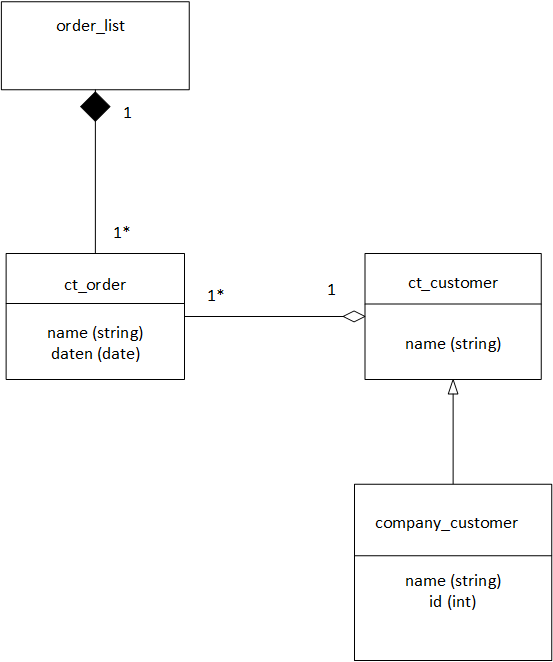
\includegraphics[scale=0.6]{1.png}

\end{center}

\noindent\textbf{3. 根据XML写XSD (10P)}

要求:

- location soll nur die Werte Chemnitz, Berlin und Paris annehmen 

- location 应该只接受 Chemnitz、Berlin 和 Paris 的值

- project muss eine eindeutige ID haben

- 项目必须有唯一的 ID

- es muss mindestens ein project geben

- 必须至少有一个项目

XML 文件如下:

\begin{minted}{xml}
<projects>
	<project id="asd2" status="in work" group="">
		<name>Test</name>
		<location>Berlin</location>
		<budget>274.12</budget>
		<conductor>
			<name>Thomas</name>
		</conductor>
	</project>
</projects> 
\end{minted}

(Die Reihenfolge der Element innerhalb von project kann variieren. Die Attribute status und group von project waren nicht immer vorhanden. 项目中元素的顺序可能会有所不同。 项目的状态和组属性并不总是存在。)
\\
\\
\textbf{4. XSLT (8P)}

XML Dokument gegeben, eine XSLT mit Lücken und die gewünschte Ausgabe. Dabei sollten E-Mails nach Priorität gruppiert werden und nur E-Mails die einen Absender von einem Dr. haben empfangen werden. Als Tipp verwenden sie starts-with( XPath, "Pattern").

给定一个 XML 文档、一个带有空缺的 XSLT 和所需的输出。 
电子邮件应根据优先级进行分组,并且仅来自博士已收到的电子邮件。 
作为提示,使用starts-with(XPath, "Pattern")。

已知的XML:

\begin{minted}{xml}
<emails>
	<inbox type="sent">
		<mail prioritaet="1">
			<absender>Dr. xy</absender>
			<datum>23-05-2000</datum>
			<betreff>xyxcyxc</betreff>
		</mail>
		<mail prioritaet="2">
			<absender>Dr. w</absender>
			<datum>21-05-2000</datum>
			<betreff>xyxcyxc</betreff>
		</mail>
	</inbox>

	<inbox type="received">
		<mail prioritaet="1">
			<absender>Dr. z</absender>
			<datum>25-05-2000</datum>
			<betreff>xyxcyxc</betreff>
		</mail>
		
		<mail prioritaet="1">
			<absender>Horst</absender>
			<datum>25-05-2000</datum>
			<betreff>xyxcyxc</betreff>
		</mail>
	</inbox>
</emails>
\end{minted}

Ausgabe:

E-Mails Priorität 1

\begin{tabular}{|c|c|c|c|}
	\hline
	Inbox & Absender&Datum&Betreff\\
	\hline
	sent&Dr.xy&23-05-2000&xyxcyxc\\
	\hline
	received&Dr.z&25-05-2000&xyxcyxc\\
	\hline
\end{tabular}

E-Mails Priorität 2

\begin{tabular}{|c|c|c|c|}
	\hline
	Inbox & Absender&Datum&Betreff\\
	\hline
	sent&Dr.w&21-05-2000&xyxcyxc\\
	\hline
\end{tabular}
\\
\\
\textbf{5. SAX (6P)}

SAX Parser erweitern, Grundgerüst gegeben und die gewünschte Ausgabe falls folgendes XML geparst wird:

扩展SAX,已知基础框架和期望的XML:

\begin{minted}{xml}
<collection shelf="blabla">
	<book title="t1">
		<author>a1</author>
	</book>
	<book title="t2">
		<author>a1</author>
	</book>
	<book title="t3">
		<author>a1</author>
	</book>
</collection>
\end{minted}

期望的输出:

\indent\indent Collection blablabla:

\indent\indent ***Book***

\indent\indent Title: t1

\indent\indent Author: a1

\indent\indent 1 of 3

\indent\indent ***Book***

\indent\indent Title: t2

\indent\indent Author: a1

\indent\indent 1 of 3

\indent\indent ***Book***

\indent\indent Title: t3

\indent\indent Author: a1

\indent\indent 1 of 3
\\
\\
\textbf{6. SPARQL (14P)}

RDF Klassen: course, student, lecturer, city

course: courseName

student: takesCourse, name, livesIn

lecturer: teaches, name, livesIn

city: cityName

SPARQL Abfragen die:

\indent a. alle Kurse ermitteln, die von Studenten besucht und von Lehrern unterrichtet werden, die aus der gleichen Stadt kommen. 确定学生参加的所有课程以及由来自同一城市的教师教授的所有课程

\indent b. alle Kurse ermitteln, die von Lehrern aus der Stadt Berlin unterrichtet werden oder deren Kursname das Wort "Engineering" enthält. 确定由柏林市教师教授的所有课程或课程名称中包含“Engineering”一词的所有课程

\textbf{Lösungsvorschlag}

a.
\begin{minted}{SPARQL}
PREFIX stud : <"http://example.org/stud#">

SELECT ?courseName
FROM ...
WHERE
{
	?course stud:courseName ?courseName.
	?teacher stud:teaches ?course.
	?student stud:takesCourse ?course.
	?student stud:livesIn ?city.
	?teacher stud:livesIn ?city.
}
\end{minted}

b.
\begin{minted}{SPARQL}
PREFIX stud : <"http://example.org/stud#">

SELECT ?courseName
FROM ...
WHERE
{
	{
		?course stud:courseName ?courseName.
		?teacher stud:teaches ?course.
		?student stud:livesIn stud:Berlin.
	}
	UNION
	{
		?course stud:courseName ?courseName.
		?teacher stud:teaches ?course.
		FILTER regex(?course_name, "Engineering")
	}
}
\end{minted}

\section{WS 2015/16}

\noindent\textbf{1. DTD (6P)}

3 XML-Files mit unterschiedlichen DTDs auf Validität überprüfen, Fehler angeben.
检查具有不同 DTD 的 3 个 XML 文件的有效性,指示错误。
\\
\\
\textbf{2. XML-Schema (10P)}

Für ein gegebenes XML-File ein passendes Schema schreiben. Bestimmte Anforderungen gegeben wie: ID muss natürliche Zahl sein, ein Element darf nur bestimmte Strings enthalten, bestimmte Attribute und deren Typen oder auch mögliche Werte sollen vorgeschrieben sein...

为给定的 XML 文件编写合适的模式。 给出了某些要求如:ID必须是自然数,一个元素只能包含某些字符串,某些属性及其类型或可能的值应该被规定...
\\
\\
\textbf{3. XSLT (10P)}

Aus der gegebenen XML-Datei sollen (geordnet nach einem Attribut "gruppe") mehrere Tabellen in XHTML ausgegeben werden.

XHTML 中的几个表将从给定的 XML 文件中输出(根据属性“组”排列)。

结果应如下图所示:

Werte innerhalb der Gruppe: GRUPPENNAME1
\begin{tabular}{|c|c|c|c|}
	\hline
	ID&Name&Info&usw\\
	\hline
	1&Muster&BlaBla&0815\\
	\hline
	2&Testmann&Etwas&42\\
	\hline
\end{tabular}

Werte innerhalb der Gruppe: GRUPPENNAME2
\begin{tabular}{|c|c|c|c|}
	\hline
	ID&Name&Info&usw\\
	\hline
	1&Tim&schon alt&02340\\
	\hline
	2&Tom&Schüler&2251\\
	\hline
	3&Tina&normal&0815\\
	\hline
\end{tabular}

Hinweis: ID muss selbst gezählt werden und keine Tabelle oder Zeile darf doppelt sein.
ID 必须单独统计,不能重复表或行。

Ein Element aus der XML-Datei könnte in etwa so aussehen XML 文件中的元素可能如下所示:

\begin{minted}{xml}
<EinElement gruppe="GRUPPENNAME1">
	<mensch>
	<name>Muster</name>
	<alter>25</alter>
	</mensch>
	<info>BlaBla</info>
	...
</EinElement>
\end{minted}

\noindent\textbf{4. SAX (6P)} Python SAX-Parser schreiben/erweitern

\noindent\textbf{5. SPARQL (14P)} FILTER() und UNION würden benötigt

\section{SS 2014}

\noindent\textbf{1. XML valid (6P)}

\begin{minted}{xml}
<?xml version="1.0"?> 
<!DOCTYPE expression [ 
	<!ELEMENT expression (term)> 
	<!ELEMENT term (wert | (term,addop,term))> 
	<!ELEMENT wert (#PCDATA)> 
	<!ELEMENT addop EMPTY> 
	<!ATTLIST addop type (plus|minus) #REQUIRED>
]> 
<expression> 
	<term> 
		<term> 
			<wert>22</wert>
		</term> 
		<addop type="minus"/> 
		<term> 
			<term><wert>55</wert></term> 
				<addop type="plus"/>
			<term><wert>14</wert></term> 
		</term> 
	</term> 
</expression>
\end{minted}

\begin{minted}{xml}
<?xml version="1.0"?> 
<!DOCTYPE expression [ 
	<!ELEMENT expression (term)> 
	<!ELEMENT term (wert | (term,addop,term))> 
	<!ELEMENT wert (#PCDATA)> 
	<!ELEMENT addop EMPTY> 
	<!ATTLIST addop type (plus|minus) #REQUIRED>
]> 
<expression> 
	<term> 
		<term>22</term> 
			<addop type="plus"/>
		<term>17</term> 
			<addop type="minus"/>
		<term>55</term> 
	</term> 
</expression>
\end{minted}

\begin{minted}{xml}
<?xml version="1.0"?> 
<!DOCTYPE expression [ 
	<!ELEMENT expression (term)> 
	<!ELEMENT term (wert | (term,addop,term))> 
	<!ELEMENT wert (#PCDATA)> 
	<!ELEMENT addop EMPTY> 
	<!ATTLIST addop type (plus|minus) #REQUIRED>
]> 
<expression> 
	<term> 
		<wert>22</wert>
	</term> 
</expression>
\end{minted}

\noindent\textbf{2. XML Schema (24P)}

已知XML-Schema和XML文件:

\begin{minted}{xml}
<?xml version="1.0" encoding="UTF-8"?> 
<xs:schema xmlns="urn:vsr:xml-pruefung:pflanzen" 
xmlns:xs="http://www.w3.org/2001/XMLSchema" 
targetNamespace="urn:vsr:xml-pruefung:pflanzen" 
elementFormDefault="qualified"> 
	<xs:element name="offers"> 
		<xs:complexType> 
			<xs:sequence maxOccurs="unbounded"> 
				<xs:element ref="product"/>
			</xs:sequence> 
		</xs:complexType>
	</xs:element> 
	<xs:complexType name="ct_planttype"> 
		<xs:sequence> 
			<xs:element name="harvest" type="xs:string"/> 
			<xs:element name="price" type="xs:double"/> 
			<xs:element name="supplier" type="xs:string"/>
		</xs:sequence> 
		<xs:attribute name="name" type="xs:string" use="required"/>
	</xs:complexType> 
	<xs:element name="product" type="ct_planttype"/> 
	<xs:complexType name="ct_fruit_planttype"> 
		<xs:complexContent> 
			<xs:extension base="ct_planttype"> 
				<xs:choice> 
					<xs:element name="stone" type="xs:boolean"/>
				</xs:choice> 
			</xs:extension> 
		</xs:complexContent>
	</xs:complexType> 
	<xs:complexType name="ct_vegtype"> 
		<xs:complexContent> 
			<xs:extension base="ct_planttype"> 
				<xs:choice> 
					<xs:element name="root" type="xs:boolean"/>
				</xs:choice> 
			</xs:extension> 
		</xs:complexContent> 
	</xs:complexType>
</xs:schema>
\end{minted}

\begin{minted}{xml}
<?xml version="1.0" encoding="UTF-8"?> 
<offers xmlns="urn:vsr:xml-pruefung:pflanzen" 
xmlns:xsi="http://www.w3.org/2001/XMLSchema-instance"> 
	<product name="nuts"> 
		<harvest>Oct</harvest> 
		<price>2.10</price> 
		<supplier>Company1</supplier>
	</product> 
	<product name="apples"> 
		<harvest>May</harvest> 
		<price>27.90</price> 
		<supplier>Company2</supplier> 
		<stone>true</stone>
	</product> 
	<product name="cabbage"> 
		<harvest>Sep</harvest> 
		<price>17.20</price> 
		<supplier>Company1</supplier> 
		<root>false</root>
	</product> 
</offers>
\end{minted}

\textbf{2a. (4) }Ändern Sie das XML File allein durch Hinzufügen von Attributen so, dass es dem Schema gemäß valide ist!
只需添加属性即可更改 XML 文件,使其根据架构有效!

\textbf{2b. (4) }Ändern Sie das Schema so, dass unter <harvest> nur noch: May, Jun, Jul und Sep angegeben werden können! Bitte schreiben Sie nicht das ganze Schema ab! Machen Sie nur kenntlich, an welchen Stellen Sie was ändern würden!
更改架构,以便在 <harvest> 下仅指定:May、Jun、Jul 和 Sep! 请不要复制整个方案! 只需明确说明您将在哪里进行更改!

\textbf{2c. (8) }Schreiben Sie eine XSL­Transformation, die Instanzen dieses Schemas (also alle zu diesem Schema validen XML­Files) in (etwa) folgende HTML­Tabelle konvertiert:
编写一个 XSLTransformation,将这个模式的实例(即所有对这个模式有效的 XML 文件)转换为(大致)以下 HTML 表:

\begin{minted}{xml}
<table border="1"> 
	<tr> 
		<th>Name</th> <th>price</th> <th>harvest</th> 
		<th>Supplier</th> <th>Type</th> 
	</tr> 
	<tr> 
		<td>nuts</td> <td>2.10</td> 
		<td>Oct</td> <td>Company1</td> 
		<td>no info</td> 
	</tr> 
	<tr> 
		<td>apples</td> <td>27.90</td> 
		<td>May</td> <td>Company2</td> <td>fruit</td> 
	</tr> 
	<tr> 
		<td>cabbage</td> <td>17.20</td> <td>Sep</td> 
		<td>Company1</td> <td>vegetable</td> 
	</tr> 
</table>
\end{minted}

\textbf{2d. (8) }Schreiben Sie eine XSL Transformation, die folgende Ausgabe erzeugt:编写产生以下输出的 XSLTransformation:

Hinweis: Die Aufgabe gilt auch dann als gelöst, wenn ein Supplier mehrfach aufgelistet wird.
注意:如果供应商被多次列出,该任务也被视为已解决。

\indent\indent The supplier Company1 supplies: nuts cabbage 

\indent\indent The supplier Company2 supplies: apples 

\indent\indent The supplier Company1 supplies: nuts cabbage
\\
\\
\textbf{3. RDF Schema, SPARQL (10P)}

已知下列RDF:

\begin{minted}{xml}
<rdf:RDF xmlns:rdf="http://www.w3.org/1999/02/22-rdf-syntax-ns#" 
	xmlns:rdfs="http://www.w3.org/2000/01/rdf-schema#" 
	xml:base="http://example.org/shop">
	<rdfs:Class rdf:ID="meal"> 
		<rdfs:comment>A meal class</rdfs:comment>
	</rdfs:Class>
	<rdf:Property rdf:ID="mealName"> 
		<rdfs:comment>The name of the meal</rdfs:comment> 
		<rdfs:domain rdf:resource="http://example.org/org#meal"/>
	</rdf:Property>
	<rdfs:Class rdf:ID="customer"> 
		<rdfs:comment>A customer class</rdfs:comment>
	</rdfs:Class>
	<rdf:Property rdf:ID="customerName"> 
		<rdfs:comment>The name the customer</rdfs:comment> 
		<rdfs:domain rdf:resource="http://example.org/org#customer" />
	</rdf:Property>
	<rdf:Property rdf:ID="prefersMeal"> 
		<rdfs:comment>A meal preferred by a customer</rdfs:comment> 
		<rdfs:domain rdf:resource="http://example.org/org#customer" /> 
		<rdfs:range rdf:resource="http://example.org/org#meal" />
	</rdf:Property> 
</rdf:RDF>
\end{minted}

Customers.rdf
\begin{minted}{xml}
<rdf:RDF 
	xmlns:rdf="http://www.w3.org/1999/02/22-rdf-syntax-ns#" 
	xmlns:shop="http://example.org/shop#" >
	<rdf:Description rdf:about="http://example.org/shop#customer2"> 
		<shop:prefersMeal rdf:resource="http://example.org/shop#meal2"/> 
		<shop:customerName>Customer2</shop:customerName>
	</rdf:Description> 
	<rdf:Description rdf:about="http://example.org/shop#customer1"> 
		<shop:prefersMeal rdf:resource="http://example.org/shop#meal3"/> 
		<shop:customerName>Customer1</shop:customerName>
	</rdf:Description> (..........................)
</rdf:RDF>
\end{minted}

Meals.rdf
\begin{minted}{xml}
<rdf:RDF 
	xmlns:rdf="http://www.w3.org/1999/02/22-rdf-syntax-ns#" 
	xmlns:shop="http://example.org/shop#" >
	<rdf:Description rdf:about="http://example.org/shop#meal0"> 
		<shop:mealName>potato</shop:mealName>
	</rdf:Description> 
	<rdf:Description rdf:about="http://example.org/shop#meal3"> 
		<shop:mealName>cherry</shop:mealName>
	</rdf:Description> (..........................)
</rdf:RDF>
\end{minted}

\textbf{3a. (4P) }Schreiben Sie eine SPARQL-­Anfrage, die herausfindet, welcher Kunde welche Mahlzeit bevorzugt!
编写一个 SPARQL 查询,找出哪个客户更喜欢哪顿饭!

Hinweis: Die Namen sollen menschenlesbar sein! (keine URLs!) 名称应该是人类可读的! (没有网址!)

\textbf{3b. (6P) }Schreiben Sie eine SPARQL­Anfrage, die alle Speisen auflistet, die sowohl vom Kunden Customer2 als auch vom Kunden Customer3 bevorzugt werden! 
编写一个 SPARQL 请求,列出客户 Customer2 和 Customer3 都喜欢的所有食物!

Hinweis 1: Die Namen sollen menschenlesbar sein! (keine URLs!) 名称应该是人类可读的! (没有网址!)

Hinweis 2: Die Aufgabe gilt auch dann als gelöst, wenn der Produktname mehrfach aufgelistet wird.
如果产品名称被多次列出,该任务也被认为已解决。

\section{SS 2013}

\textbf{1.XML valid (6P)}

\begin{minted}{xml}
<?xml version="1.0" encoding="UTF-8"?>
<!DOCTYPE expression [
  	<!ELEMENT expression  (term)>  
  	<!ELEMENT term  (wert | (term,addop,term))>  
	<!ELEMENT wert  (#PCDATA)>
  	<!ELEMENT addop  EMPTY>
  	<!ATTLIST addop type (plus|minus) #REQUIRED>
]>
<!-- INVALID -->
<expression>
  	<term>
   	 	<term>22</term>
      		<addop type="plus"/>
    	<term>17</term>
      		<addop type="minus"/>
    	<term>55</term>
  	</term>
</expression>
\end{minted}

\begin{minted}{xml}
<?xml version="1.0" encoding="UTF-8"?>
<!DOCTYPE expression [
  	<!ELEMENT expression  (term)>	
  	<!ELEMENT term  (wert | (term,addop,term))>	
  	<!ELEMENT wert  (#PCDATA)>
  	<!ELEMENT addop  EMPTY>
  	<!ATTLIST addop type (plus|minus) #REQUIRED>
]>
<!-- INVALID -->
<expression>
  	<term>
    	<wert>22</wert>
  	</term>
</expression>
\end{minted}

\begin{minted}{xml}
<?xml version="1.0" encoding="UTF-8"?>
<!DOCTYPE expression [
  	<!ELEMENT expression  (term)>	
  	<!ELEMENT term  (wert | (term,addop,term))>	
  	<!ELEMENT wert  (#PCDATA)>
  	<!ELEMENT addop  EMPTY>
  	<!ATTLIST addop type (plus|minus) #REQUIRED>
]>
<!-- VALID -->
<expression>
  	<term>
    	<term>
      		<wert>22</wert>
    	</term>
    	<addop type="minus"/>
    	<term>
      		<term><wert>55</wert></term>
        		<addop type="plus"/>
      		<term><wert>14</wert></term>
    	</term>
  	</term>
</expression>
\end{minted}

\noindent\textbf{2. XML Schema, XSD}

Ist das XML-File gegen das gegebene Schema valid?  (2 Punkte)

(4 Punkte) wenn ja: machen sie irgendwas (weis ich nicht, war nicht der Fall) 

wenn nein: Wie kann das XML-File durch einfügen eines einzigen Attributes valid gemacht werden?

\begin{minted}{xml}
<?xml version="1.0" encoding="UTF-8"?>
<xs:schema xmlns:xs="http://www.w3.org/2001/XMLSchema" 
	elementFormDefault="qualified">

  	<xs:element name="animals">
    	<xs:complexType>
      		<xs:sequence>
        		<xs:element ref="animal" minOccurs="1" maxOccurs="unbounded"/>
      		</xs:sequence>
    	</xs:complexType>
  	</xs:element>

  	<xs:complexType name="ct_animal">
    	<xs:sequence>
      		<xs:element name="speed" type="xs:double"/>
    	</xs:sequence>
    	<xs:attribute name="name" type="xs:string" use="required"/>
  	</xs:complexType>
  
  	<xs:complexType name="ct_bird">
    	<xs:complexContent>
      	<xs:extension base="ct_animal">
        	<xs:sequence>
          		<xs:element name="flughöhe_oder_so" type="xs:double"/>
        	</xs:sequence>
      	</xs:extension>
    	</xs:complexContent>
  	</xs:complexType>

  	<xs:element name="animal" type="ct_animal"/>
  
</xs:schema>
\end{minted}

\begin{minted}{xml}
<?xml version="1.0" encoding="UTF-8"?>

<animals>
  	<animal name="eagle">
    	<speed>120.0</speed>
    	<flughöhe_oder_so>700.0</flughöhe_oder_so>
  	</animal>
  	<animal name="horse">
    	<speed>45.0</speed>
  	</animal>
</animals>

<!--
Teilaufgabe 2.2

<animals>
  	<animal name="eagle" xsi:type="ct_bird">
    	<speed>120.0</speed>
    	<flughöhe_oder_so>700.0</flughöhe_oder_so>
  	</animal>
  	<animal name="horse">
    	<speed>45.0</speed>
  	</animal>
</animals>
-->
\end{minted}

\noindent\textbf{3. XSD -> XML (20P)}

为warehouses.xsd文件撰写一个有效的XML样式表

\begin{minted}{xml}
<?xml version="1.0" encoding="UTF-8"?>
<xs:schema xmlns:xs="http://www.w3.org/2001/XMLSchema" 
	elementFormDefault="qualified">
  	<xs:element name="warehouses">
    	<xs:complexType>
      		<xs:sequence>
        		<xs:element ref="warehouse" maxOccurs="unbounded"/>
      		</xs:sequence>
    	</xs:complexType>
  	</xs:element>
  
  	<xs:element name="warehouse">
    	<xs:complexType>
      		<xs:sequence>
       	 		<xs:element name="Item" maxOccurs="unbounded">
          			<xs:complexType>
            			<xs:all>
              				<xs:element name="Name" type="xs:string"/>
              				<xs:element name="price" type="xs:double"/>
            			</xs:all>
          			</xs:complexType>
        		</xs:element>
      		</xs:sequence>
      		<xs:attribute name="name" type="xs:string" use="required"/>
    	</xs:complexType>
  	</xs:element>
</xs:schema>
\end{minted}

产生以下输出:

\begin{minted}{xml}
<table border="1">
	<tr> <th> Name </th> <th> price </th> <th> warehouse </th> </tr>
	<tr> <td> Bla1 </td>  <td> 1000.0</td> <td> Warehouse1 </td></tr>
	<tr> <td> Bla2 </td>  <td> 3000.0</td> <td> Warehouse1 </td></tr>
	<tr> <td> Bla3 </td>  <td> 4000.0</td> <td> Warehouse1 </td></tr>
	<tr> <td> Bla4 </td>  <td> 5000.0</td> <td> Warehouse2 </td></tr>
	<tr> <td> Bla5 </td>  <td> 6000.0</td> <td> Warehouse2 </td></tr>
	<tr> <td> Bla6 </td>  <td> 7000.0</td> <td> Warehouse3 </td></tr>
	(...)
</table>
\end{minted}

\textbf{3a. } 并输出每件商品的Name, price, warehouse。

\textbf{3b. } Geben Sie die Namen aller Items aus, die es in mehreren Warenhousern gibt.
打印出多个仓库中存在的所有物品的名称。

注意!:如果物品被多次给予,该任务也被视为已解决。

\textbf{Lösungen}

3a.
\begin{minted}{xml}
<?xml version="1.0" encoding="UTF-8"?>
<xsl:stylesheet xmlns:xsl="http://www.w3.org/1999/XSL/Transform" version="1.0">

  	<xsl:template match="/">
    	<table border="1">
      		<tr>
        		<th>Name</th><th>price</th><th>warehouse</th>
      		</tr>
      		<xsl:apply-templates select="warehouse"/>
    	</table>
  	</xsl:template>

  	<xsl:template match="warehouse">
    	<xsl:variable name="w_name" select="@name"/>
    	<xsl:for-each select="Item">
      		<tr>
        		<td><xsl:value-of select="Name/text()"/></td>
        		<td><xsl:value-of select="price/text()"/></td>
        		<td><xsl:value-of select="$w_name"/></td>
      		</tr>
    	</xsl:for-each>
  	</xsl:template>
</xsl:stylesheet>
\end{minted}

3b.

\begin{minted}{xml}
<?xml version="1.0" encoding="UTF-8"?>
<xsl:stylesheet xmlns:xsl="http://www.w3.org/1999/XSL/Transform" version="1.0">
  
  	<xsl:template match="//warehouse">
    	<xsl:variable name="W_name" select="@name"/>
    	<xsl:for-each select="Item">
      		<xsl:call-template name="doppelt">
        		<xsl:with-param name="w_name" select="$W_name"/>
        		<xsl:with-param name="Item_n" select="Name/text()"/>
      		</xsl:call-template>
    	</xsl:for-each>
  	</xsl:template>
  
  	<xsl:template name="doppelt">
    	<xsl:param name="w_name"/>
    	<xsl:param name="Item_n"/>
    	<xsl:for-each select="//warehouse[not(@name = $w_name)]">
      		<xsl:for-each select="Item[Name/text() = $Item_n]">
        		<p><xsl:value-of select="Name/text()"/></p>
      		</xsl:for-each>
    	</xsl:for-each>
  	</xsl:template>
</xsl:stylesheet>
\end{minted}

\noindent\textbf{4. SPARQL (12P)}

prod\_rdf\_schema.xml

\begin{minted}{xml}
<?xml version="1.0" encoding="UTF-8"?>

<!-- könnte was fehlen -->

<rdf:RDF xmlns:rdf="http://www.w3.org/1999/02/22-rdf-syntax-ns#"
        xmlns:rdfs="http://www.w3.org/2000/01/rdf-schema#"
        xmlns="http://example.org/sup#"
>
  	<rdfs:Class rdf:ID="producer">
      	<rdfs:comment>A producer bla</rdfs:comment>
  	</rdfs:Class>

  	<rdfs:Class rdf:ID="product">
      	<rdfs:comment>A product bla</rdfs:comment>
  	</rdfs:Class>

  	<rdf:Property rdf:ID="productName">
      	<rdfs:comment>The name of the product</rdfs:comment>
      	<rdfs:domain rdf:resource="http://example.org/lit#product"/>
  	</rdf:Property>

  	<rdf:Property rdf:ID="producerName">
      	<rdfs:comment>The name the producer</rdfs:comment>
      	<rdfs:domain rdf:resource="http://example.org/lit#producer" />
  	</rdf:Property>

  	<rdf:Property rdf:ID="hasProduced">
      	<rdfs:comment>A product produced by a producer</rdfs:comment>
      	<rdfs:domain rdf:resource="http://example.org/lit#producer" />
      	<rdfs:range rdf:resource="http://example.org/lit#product" />
  	</rdf:Property>
</rdf:RDF>
\end{minted}

producers\_products\_rdf.xml
\begin{minted}{xml}
<?xml version="1.0" encoding="UTF-8"?>
<!-- Producers.rdf

      könnte statt
      http://example.org/sup# productX
      auch
      http://example.org/sup# articelX
      sein
-->
<rdf:RDF
    xmlns:sup="http://example.org/sup#"
    xmlns:rdf="http://www.w3.org/1999/02/22-rdf-syntax-ns#" 
> 
  	<rdf:Description rdf:about="http://example.org/sup#producer0">
    	<sup:hasProduced rdf:resource="http://example.org/sup#product0"/>
    	<sup:producerName>Producer 1</sup:producerName>
  	</rdf:Description>
  	<rdf:Description rdf:about="http://example.org/sup#producer1">
    	<sup:hasProduced rdf:resource="http://example.org/sup#product1"/>
    	<sup:producerName>Producer 1</sup:producerName>
  	</rdf:Description>
  	<rdf:Description rdf:about="http://example.org/sup#producer2">
		<sup:hasProduced rdf:resource="http://example.org/sup#product2"/>
		<sup:hasProduced rdf:resource="http://example.org/sup#product3"/>
		<sup:producerName>Producer 2</sup:producerName>
	</rdf:Description>
	<rdf:Description rdf:about="http://example.org/sup#producer3">
		<sup:hasProduced rdf:resource="http://example.org/sup#product3"/>
		<sup:producerName>Producer 3</sup:producerName>
	</rdf:Description>
</rdf:RDF>

<!-- Products.rdf 
      könnte statt
      http://example.org/sup# productX
      auch
      http://example.org/sup# articelX
      sein;
      und nochmal der Hinweis: vielleicht fehlt noch was
-->
<rdf:RDF
    xmlns:sup="http://example.org/sup#"
    xmlns:rdf="http://www.w3.org/1999/02/22-rdf-syntax-ns#" 
> 
	<rdf:Description rdf:about="http://example.org/sup#product0">
		<sup:productName>Product 0</sup:productName>
	</rdf:Description>
	<rdf:Description rdf:about="http://example.org/sup#product1">
		<sup:productName>Product 1</sup:productName>
	</rdf:Description>
	<rdf:Description rdf:about="http://example.org/sup#product2">
		<sup:productName>Product 2</sup:productName>
	</rdf:Description>
	<rdf:Description rdf:about="http://example.org/sup#product3">
		<sup:productName>Product 3</sup:productName>
	</rdf:Description>
</rdf:RDF>
\end{minted}

\textbf{4a. } Geben Sie mit Hilfe einer SPARQL-Anfrage die Produzenten und zu jedem Produzent seine Produkte aus! (4 Punkte)
使用 SPARQL 查询为每个生产者输出生产者及其产品!

注意:它不应该是 URL,而是输出的名称。

\begin{minted}{SPARQL}
Prefix sup: <http://example.org/sup#>
Select ?producer_name ?product_name
From <Producers.rdf>
From <Products.rdf>
Where {
	?producer sup:hasProduced ?product .
	?producer sup:producerName ?producer_name .
	?product  sup:productName  ?product_name .
}
\end{minted}

\textbf{4b. } Geben Sie mit Hilfe einer SPARQL-Anfrage diejenigen Produkte aus, die sowohl von producer2 als auch von producer3 produziert wurden!
(8 Punkte) 使用 SPARQL 查询返回 producer2 和 producer3 生产的产品!

\begin{minted}{SPARQL}
Prefix sup: <http://example.org/sup#>
Select ?product_name
From <Producers.rdf>
From <Products.rdf>
Where {
	sup:producer2 sup:hasProduced ?product .
	sup:producer3 sup:hasProduced ?product . 
	?product  sup:productName  ?product_name .
}
\end{minted}


\newpage

\part*{Zusammenfassung}

\setcounter{section}{0}

\section{lb1: Validation: DTD, XML-Schema(.xsd), UML }

\subsection{概念}

F1: 什么是Validation?

A1: Validation \dots

\indent\indent fixes wrong XML files 修复错误的 XML 文件

\indent\indent compares XML files to an expected structure 将 XML 文件与预期的结构进行比较($\checkmark$)

\indent\indent is pre-requisite for reading data from XML files 是从 XML 文件读取数据的先决条件

\indent\indent decodes XML files 解码 XML 文件

F2: 什么是DTD?

A2: DTD \dots

\indent\indent enables easy reuse of element declarations across documents 可以轻松地跨文档重用元素声明

\indent\indent has many data types 有很多数据类型

\indent\indent can be in the same document as the corresponding XML instance data 可以和对应的 XML 实例数据在同一个文档中($\checkmark$)

\indent\indent has the same syntax as XML documents 具有与 XML 文档相同的语法

F3: 什么是XML Schema?

A3: XML Schema \dots

\indent\indent is always shorter than an equivalent DTD 总是比等效的 DTD 短

\indent\indent requires a dedicated separate parser 需要一个专用的独立解析器

\indent\indent is limited to a list of pre-defined data types 仅限于预定义数据类型的列表

\indent\indent does not explicitly specify the root element 没有明确指定根元素($\checkmark$)

F4: 判断:A single-element (self-closed) document can be well-formed. 单元素(自闭合)文档可以是格式良好的。

A4: True ($\checkmark$)/ False

F5: With XSD you cannot\dots

A5: 

\indent\indent restrict the content of strings. 限制字符串的内容。

\indent\indent add attributes to elements with simple content.为内容简单的元素添加属性。

\indent\indent define entities. 定义实体。($\checkmark$)

\indent\indent define an element with recursive content. 定义具有递归内容的元素。

\subsection{XML和HTML的区别}

1. HTML的标签不能自定义,XML的标签必须自定义。HTML-Tags können nicht angepasst werden, XML-Tags müssen angepasst werden.

2. HTML语法要求不严格,XML语法要求极其严格——必须是成对标签。Die Anforderungen an die HTML-Syntax sind nicht streng, die Anforderungen an die XML-Syntax sind extrem streng - müssen gepaarte Tags sein.

3. XML用来传输或存储数据,HTML用来展示数据。XML wird zum Übertragen oder Speichern von Daten verwendet, HTML zum Anzeigen von Daten.

\subsection{XML语法规则}

1. XML必须有根结点——是其他所有节点的父节点。XML muss einen Stammknoten haben – den übergeordneten Knoten aller anderen Knoten

2. XML的头声明:不强制。XML-Header-Deklaration: nicht obligatorisch

3. 所有XML元素都必须是成对标签。Alle XML-Elemente müssen gepaarte Tags sein

4. 标签名大小写敏感。Bei Tag-Namen wird zwischen Groß- und Kleinschreibung unterschieden

5. 标签不能交叉。Labels können sich nicht kreuzen

6. 符号要用实体转义,Symbole sollten mit Entities maskiert werden:

\begin{center}
\begin{tabular}{|c|c|c|}
	\hline
	\&lt; & < & 小于\\
	\hline
	\&gt; & > & 大于\\
	\hline
	\&amp; & \& & 和号\\
	\hline
	\&apos; & ' & 单引号\\
	\hline
	\&quot; & " & 双引号\\
	\hline
\end{tabular}
\end{center}

\subsection{DTD 约束 (.dtd)}

使用DTD文当前,必须将以下代码导入到目标文件中(第二行)
\begin{center}
	\begin{minted}{xml}
		<!DOCTYPE 根元素 SYSTEM "路径/文档1.dtd" >
	\end{minted}
\end{center}

若引用的DTD文件是一个公共的文件时,采用PUBLIC标示,如下:

\begin{center}
	\begin{minted}{xml}
		<!DOCTYPE 根元素 PUBLIC "DTD名称" "DTD文件的URL">
	\end{minted}
\end{center}

\subsubsection{DTD 例子}

\begin{minted}{xml}
<?xml version="1.0" encoding="utf-8"?>
<!DOCTYPE root[
	<!ELEMENT root (node1*, node2*, node3?)>
	<!ELEMENT node1 (node4+)>
	<!ELEMENT node4 (#PCDATA)>

	<!ATTLIST node2
		属性名称 类型 特点
	>
]>
\end{minted}

\noindent 其中小括号内的符号与模式匹配相同:

1. $?$: 在父标签内出现$0~1$次;

2. $+$: 在父标签内出现$1~\infty$

3. \#PCDATA: 没有子标签

4. $*$: 出现$0~\infty$

5. 没有多与符号: 必须且仅能出现1次

6. (子标签1|子标签2): 二者至少出现其一,也可同时出现

7. 子标签的顺序是不可更改的,例如上方node1必须出现在node2和node3之前。

8. 若标签名后面跟的是EMPTY: 表示该元素不包含子元素和文本,但可以有属性

9. 若标签后面跟的是ANY: 可以包含任何该DTD中定义的元素内容
\\
\\
在属性ATTLIST中,类型有5种:

1. CDATA: 可以使用任何字符

2. ID: 表示该属性的取值必须唯一

3. IDREF/IDREFS: 该属性的值指向文档中其他地方声明的ID类型的值,IDREFS与IDREF类似,但可以具有由空格分隔开的多个引用:

\begin{minted}{xml}
<?xml version="1.0" encoding="utf-8"?>
<!DOCTYPE person[
	<!ELEMENT person(人)>

	<!ATTLIST 人
		nr ID #REQUIRED
		parentID IDREFS #IMPLIED
		name CDATA #REQUIRED	
	>
]>
<person>
	<人 nr="P_1" name="王父"/>
	<人 nr="P_2" name="王母"/>
	<人 nr="P_3" parentID="P_1 P_2" name="王仔"/>
</person>
\end{minted}

4. Enumerated: 事先定义好一些值,属性的值必须在所列出的值的范围内(类似枚举):

\begin{minted}{xml}
...
	<!ATTLIST person
		婚姻状态 (single|married|divorced|widowed) #IMPLIED
		性别 (男|女) #REQUIRED
	>
...
\end{minted}

5. ENTITY/ENTITIES: 实体。为一段内容创建一个别名,以后在XML文档中就可以使用该别名来引用。实体分两种:

\indent\indent 5.1 引用实体:是被XML文档应用的;引用方式:\&实体名称;
\begin{minted}{xml}
...
	<!ENTITY copyright "I am a programmer">
...
	&copyright;
...
\end{minted}

\indent\indent 5.2 参数实体:被DTD文件本身应用的。引用方式:\%实体名称;

\begin{minted}{xml}
...
	<!ENTITY % TAG_NAME "姓名|EMAIL|电话|地址">
	<!ENTITY 个人信息 (%TAG_NAME;|生日)>
    <!ENTITY 客户信息 (%TAG_NAME;|公司名)>
...
\end{minted}

\noindent 属性的特点有4中:

1. \#REQUIRED: 必须有

2. \#IMPLIED: 可选

3. \#FIXED value: 必须有一个固定的value值

4. Default value: 如果这个属性没有值,那么就分配一个默认的value值

\textbf{但在XML中不推荐使用属性,因为在解析XML数据时,属性会带来额外的解析代码。}

\subsection{CDATA}

在XML中存在语义转换,有时会造成麻烦,因此为了解决这个问题,可以使用CDATA的方法“不解析”字符。

\begin{minted}{xml}
...
	<xsl:text><![CDATA[1 & 1 = true, 2 > 1]]></xsl:text>
...
\end{minted}

\subsection{Schema 约束 (.xsd)}

在使用Schema约束之前,必须将以下代码导入到目标文件中:

\begin{minted}{xml}
<?xml version="1.0" encoding="UTF-8"?>
<root xmlns="______1______"
	  xmlns:xsi="http://www.w3.org/2001/XMLSchema-instance"
	  xsi:schemaLocation="_______2______ 路径/约束文件名称.xsd"
>
	...
</root>
\end{minted}

而在.xsd文件中,需要写为:

\begin{minted}{xml}
<?xml version="1.0" encoding="UTF-8"?>
<xs:schema xmlns="______3______"
		   xmlns:xs="http://www.w3.org/2001/XMLSchema"
		   targetNamespace="______4______"
		   elementFormDefault="qualified"
>
...
</xs:schema>
\end{minted}

4(targetNamespace): 该schema定义的元素所来自的命名空间,它可以是外部,也可以是自定名称。当为自定名称时,表示来自自己。

3(xmlns): 指出默认的命名空间,影响targetNamespace,在.xsd中,当为3为自订时,4=3。

2(xsi:schemaLocation): 为命名空间的名字,也就是2=3。

1(xmlns): 与3类似,指出默认的命名空间,对于xml来说,就是其schema文件的命名空间,也就是说,1=3。

xmlns:xsi="http://www.w3.org/2001/XMLSchema-instance": 一旦有了可用的XML Schema,命名空间将被实例化。

xmlns:xs="http://www.w3.org/2001/XMLSchema": 显示schema中用到的元素和数据类型来自此命名空间。该命名空间规定了元素和数据类型应使用前缀\textbf{xs:}

elementFormDefault="qualified": 指出任何XML实例文档所使用的,且在此schema中声明过的元素必须被命名空间限定。

\subsubsection{xs:simplyType 简单类型}

指仅包含文本的元素,它不会包含任何其他的元素或属性。

\begin{minted}{xml}
<xs:element name="..." type="..." />	
\end{minted}

其中type常见的有:

\indent\indent xs:string

\indent\indent xs:decimal

\indent\indent xs:integer

\indent\indent xs:boolean

\indent\indent xs:date

\indent\indent xs:time

在声明一个简单类型时,还可以添加默认值或固定值:

\begin{minted}{xml}
	<!--默认值-->
	<xs:element name="color" type="xs:string" default="red" />
	<!--固定值-->
	<xs:element name="color" type="xs:string" fixed="red" />
\end{minted}

\subsubsection{xs:attribute 属性}

简单类型无法拥有属性。但属性本身是作为简单类型声明的。

\begin{minted}{xml}
	<xs:attribute name="..." type="..." />
\end{minted}

其中type与简单类型中的相同。此外也能设定默认值和固定值

此外,默认情况下,属性是可选的。如果要规定属性为必选,需要用到\textbf{use}:

\begin{minted}{xml}
	<xs:attribute name="lang" type="xs:string" use="required"/>
\end{minted}

\subsubsection{xs:restriction 限定}

可以对元素进行限制

\begin{minted}{xml}
<!--对单个值age的限定为[0,120]-->
<xs:element name="age">
	<xs:simpleType>
		<xs:restriction base="xs:integer">
			<xs:minInclusive value="0"/>
			<xs:maxInclusive value="120"/>
		</xs:restriction>
	</xs:simpleType>
</xs:element>

<!--将car的内容限定为一组可接受的值,用枚举约束enumeration constraint-->
<xs:element name="car">
	<xs:simpleType>
		<xs:restriction base="xs:string">
			<xs:enumeration value="Audi"/>
			<xs:enumeration value="Golf"/>
			<xs:enumeration value="BMW"/>
		</xs:restriction>
	</xs:simpleType>
</xs:element>

<!--还可以这么写。在这种情况下carType还可以被更多元素调用-->
<xs:element name="car" type="carType"/>
<xs:simpleType name="carType">
	<xs:restriction base="xs:string">
		<xs:enumeration value="Audi"/>
		<xs:enumeration value="Golf"/>
		<xs:enumeration value="BMW"/>
	</xs:restriction>
</xs:simpleType>

<!--限定为小写字母-->
...
	<xs:restriction base="xs:string">
		<xs:pattern value="[a-z]"/>
...

<!--限定为小写字母串-->
...
	<xs:restriction base="xs:string">
		<xs:pattern value="([a-z])*"/>
...

<!--限定"或"-->
...
	<xs:restriction base="xs:string">
		<xs:pattern value="male|female"/>
...

<!--预留空白-->
...
		<xs:whiteSpace value="preserve"/>
...

<!--移除所有空白/换行/回车/制表符-->
...
		<xs:whiteSpace value="replace"/>
...

<!--替换所有空白/换行/回车/制表符为单个空格-->
...
		<xs:whiteSpace value="collapse"/>
...

<!--限定字符长度-->
...
		<xs:length value="8"/>
...
\end{minted}

\subsubsection{xs:complexType 复杂类型}

包含其他元素/属性的元素。

\begin{minted}{xml}
<!--不可复用-->
<xs:element name="元素名称">
	<xs:complexType>
		...
	</xs:complexType>
</xs:element>

<!--可复用-->
<xs:element name="元素名称" type="自定义类型1"/> 

<xs:complexType name="自定义类型2">        
	(其他成分) 
</xs:complexType>  

<xs:complexType name="自定义类型1">          
	<xs:complexContent>                   
		<xs:extension base="自定义类型2">                            
			(其他成分)              
 		</xs:extension>         
 	</xs:complexContent> 
</xs:complexType>
<!--上面xs:extension部分,是扩展了自定义类型2-->
\end{minted}

\noindent\textbf{.xsd 实例}

\begin{minted}{xml}
<!--空元素:不包含内容,只有属性,如<product prodid="1345"/>-->
<xs:element name="product" type="productType"/>
<xs:complexType name="productType">
	<xs:attribute name="prodid" type="xs:positiveInteger" />
</xs:complexType>

<!--仅含元素:只能包含其他元素的元素。
xs:sequence是指示器,保证了子元素必须按照特定的顺序出现
形如: 
<person>
	<firstname>John</firstname>
	<lastname>Smith</lastname>
</person> -->
<xs:element name="person" type="personType"/>
<xs:complexType name="personType">
	<xs:sequence>
		<xs:element name="firstname" type="xs:string"/>
		<xs:element name="lastname" type="xs:string"/>
	</xs:sequence>
</xs:complexType>

<!--仅包含文本和属性,如 <firstname por="3">John</firstname>-->
<xs:element name="firstname" type="firstnameType"/>
<xs:complexType name="firstnameType">
	<xs:simpleContent>
		<xs:extension base="xs:string">
			<xs:attribute name="por" type="xs:positiveInteger"/>
		</xs:extension>
	</xs:simpleContent>
</xs:complexType>

<!--全都有。其中mixed=true保证了字符数据出现在子元素之间
<letter>
	Dear Mr. <name>John Smith</name>.
	Your order <orderid>1032</orderid>
	will be shipped on <shipdate>2001-07-13</shipdate>.
</letter>
-->
<xs:element name="letter" type="letterType"/>
<xs:complexType name="letterType" mixed="true">
	<xs:sequence>
		<xs:element name="name" type="xs:string"/>
		<xs:element name="orderid" type="xs:positiveInteger"/>
		<xs:element name="shipdate" type="xs:date"/>
	</xs:sequence>
</xs:complexType>

<!--指示器:用于指定元素的顺序-->
<!--xs:all  子元素可以按照任意顺序出现,且必须只出现1次-->
<xs:element name="person" type="personType"/>
<xs:complexType name="personType">
	<xs:all>
		<xs:element name="firstname" type="xs:string"/>
		<xs:element name="lastorderid" type="xs:string"/>
	</xs:all>
</xs:complexType>

<!--xs:choice  多选1-->
<xs:element name="person">
	<xs:complexType>
		<xs:choice>
			<xs:element name="employee" type="xs:string"/>
			<xs:element name="boss" type="xs:string"/>
		</xs:choice>
	</xs:complexType>
</xs:element>

<!--occurrence指示器:规定某个元素出现的频率
maxOccurs默认为1,若想不受限,用maxOccurs="unbounded"
minOccurs默认为1
-->
<xs:element name="position" type="xs:positiveInteger" maxOccurs="10" minOccurs="0">

<!--group指示器:用于定义相关的数个元素。必须在其内部定义一个all/choice/sequence-->
<!--调用是,用ref进行引用-->
<xs:group name="persongroup">
	<xs:sequence>
		<xs:element name="firstname" type="xs:string" />
		<xs:element name="lastname" type="xs:string" />
		<xs:element name="birthday" type="xs:date" />
	</xs:sequence>
</xs:group>

<xs:element name="person" type="personinfo" />
<xs:complexType name="personinfo">
	<xs:sequence>
		<xs:group ref="persongroup" />
		<xs:element name="country" type="xs:string" />
	</xs:sequence>
</xs:complexType>

<!--属性组,与group类似,也需要用ref引用-->
<xs:attributeGroup name="personattrgroup">
	<xs:attribute name="firstname" type="xs:string" />
	<xs:attribute name="lastname" type="xs:string" />
	<xs:attribute name="birthday" type="xs:date" />
</xs:attributeGroup>

<xs:element name="person">
	<xs:complexType>
		<xs:attributeGroup ref="personattrgroup" />
	</xs:complexType>
</xs:element>
\end{minted}

\subsection{根据UML写XSD,以及配套一个实例XML}

已知UML图:

\begin{center}
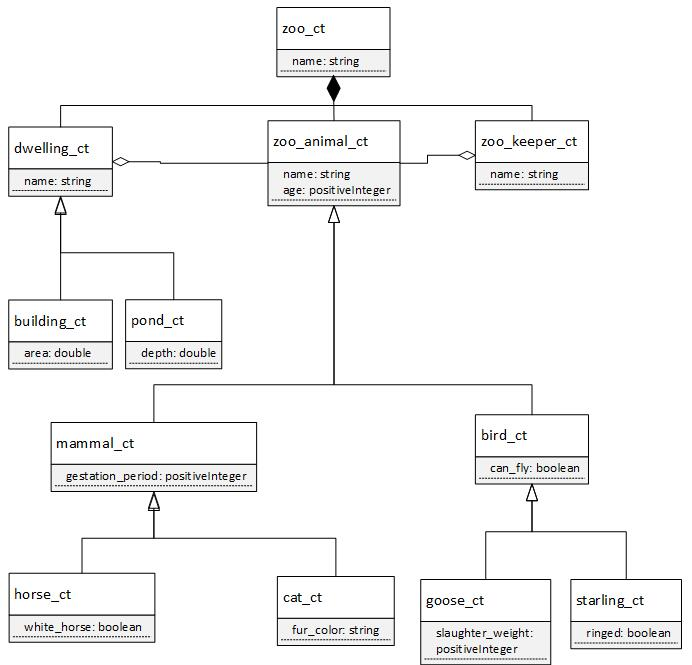
\includegraphics[scale=0.8]{9.jpg}
\end{center}

可能的.xsd文件为:

\begin{minted}{xml}
<?xml version="1.0" encoding="UTF-8" ?>
<xs:schema xmlns="xsd18" 
    xmlns:xs="http://www.w3.org/2001/XMLSchema"
    targetNamespace="xsd18"
    elementFormDefault="qualified"
>
    <!-- 根元素 -->
    <xs:element name = "zoo">
        <xs:complexType>
            <xs:all>
                <xs:element ref="dwelling"/>
                <xs:element ref="zoo_animal"/>
                <xs:element ref="zoo_keeper"/>
            </xs:all>
        </xs:complexType>
    </xs:element>

    <!-- 根的子元素 -->
    <xs:element name="dwelling" type = "dwelling_ct"></xs:element>
    <xs:element name="zoo_animal" type = "zoo_animal_ct"></xs:element>
    <xs:element name="zoo_keeper" type = "zoo_keeper_ct"></xs:element>

    <!-- 根的子元素类型1 -->
    <xs:complexType name="dwelling_ct">
        <xs:sequence>
            <xs:element name="id" type = "xs:ID" />
            <xs:element name="name" type = "xs:string" />
        </xs:sequence>
    </xs:complexType>
    <!-- 根的子元素类型1 的 子元素类型1 -->
    <xs:complexType name="building_ct">
        <xs:complexContent>
            <xs:extension base = "dwelling_ct">
                <xs:choice>
                    <xs:element name="area" type = "xs:double" />
                </xs:choice>
            </xs:extension>
        </xs:complexContent>
    </xs:complexType>
    <!-- 根的子元素类型1 的 子元素类型2 -->
    <xs:complexType name="pond_ct">
        <xs:complexContent>
            <xs:extension base = "dwelling_ct">
                <xs:choice>
                    <xs:element name="depth" type = "xs:double" />
                </xs:choice>
            </xs:extension>
        </xs:complexContent>
    </xs:complexType>

    <!-- 根子元素类型2 -->
    <xs:complexType name="zoo_animal_ct">
        <xs:sequence>
            <xs:element name="id" type = "xs:ID" />
            <xs:element name="name" type="xs:string" />
            <xs:element name="age" type="xs:positiveInteger" />
        </xs:sequence>
        <xs:attribute name="dwelling" type = "xs:IDREF" use = "required"/>
        <xs:attribute name="zoo_keeper" type = "xs:IDREF" use = "required"/>
    </xs:complexType>
    <!-- 根子元素类型2 的 子元素类型1 -->
    <xs:complexType name="mammal_ct">
        <xs:sequence>
            <xs:element name="gestation_period" type = "xs:positiveInteger" />
        </xs:sequence>
    </xs:complexType>
    <!-- 根子元素类型2 的 子元素类型1 的 子元素类型1 -->
    <xs:complexType name="horse_ct">
        <xs:complexContent>
            <xs:extension base="mammal_ct">
                <xs:choice>
                    <xs:element name="white_horse" type="xs:boolean" />
                </xs:choice>
            </xs:extension>
        </xs:complexContent>
    </xs:complexType>
    <!-- 根子元素类型2 的 子元素类型1 的 子元素类型2 -->
    <xs:complexType name="cat_ct">
        <xs:complexContent>
            <xs:extension base="mammal_ct">
                <xs:choice>
                    <xs:element name="fur_color" type="xs:string" />
                </xs:choice>
            </xs:extension>
        </xs:complexContent>
    </xs:complexType>

    <!-- 根子元素类型2 的 子元素类型2 -->
    <xs:complexType name="bird_ct">
        <xs:sequence>
            <xs:element name="can_fly" type = "xs:boolean" />
        </xs:sequence>
    </xs:complexType>

    <!-- 根子元素类型2 的 子元素类型2 的 子元素类型1 -->
    <xs:complexType name="goose_ct">
        <xs:complexContent>
            <xs:extension base="bird_ct">
                <xs:choice>
                    <xs:element name="slaughter_weight" type="xs:positiveInteger" />
                </xs:choice>
            </xs:extension>
        </xs:complexContent>
    </xs:complexType>
    <!-- 根子元素类型2 的 子元素类型2 的 子元素类型2 -->
    <xs:complexType name="starling_ct">
        <xs:complexContent>
            <xs:extension base="bird_ct">
                <xs:choice>
                    <xs:element name="ringed" type="xs:boolean" />
                </xs:choice>
            </xs:extension>
        </xs:complexContent>
    </xs:complexType>

    <!-- 根子元素类型3 -->
    <xs:complexType name="zoo_keeper_ct">
        <xs:sequence>
            <xs:element name="id" type = "xs:ID" />
            <xs:element name = "name" type = "xs:string"/>
        </xs:sequence>
    </xs:complexType>

</xs:schema>
\end{minted}

对应的xml实例:
\begin{minted}{xml}
<?xml version="1.0" encoding="UTF-8"?>
<zoo xmlns="xsd18"
    xmlns:xsi="http://www.w3.org/2001/XMLSchema-instance"
    xsi:schemaLocation="xsd18 xsd18.xsd"
>

    <dwelling xsi:type="building_ct">
        <id>a1</id>
        <name>a</name>
        <area>1.1</area>
    </dwelling>

    <zoo_keeper>
        <id>b1</id>
        <name>b</name>
    </zoo_keeper>

    <zoo_animal dwelling="a1" zoo_keeper="b1">
        <id>c1</id>
        <name>ani1</name>
        <age>11</age>
    </zoo_animal>

</zoo>
\end{minted}


\section{lb2: SAX, DOM (.py)}

\subsection{概念}

判断:
F1: Data Processing...

\indent\indent can only be done using a SAX or DOM parser 只能使用 SAX 或 DOM 解析器完成

\indent\indent can only happen on already validated files 只能发生在已经验证的文件上

\indent\indent creates XML data from HTTP forms 从 HTTP 表单创建 XML 数据

\indent\indent reads structured data for use in an application 读取结构化数据以在应用程序中使用($\checkmark$)

F2: SAX Parser...

\indent\indent are a W3C recommended standard 是 W3C 推荐的标准

\indent\indent can not access attributes 不能访问属性

\indent\indent don't need to load the entire document into memory 不需要将整个文档加载到内存中($\checkmark$)

\indent\indent provide methods to follow ID-references easily 提供了容易地遵循 ID 引用的方法

F3: An XML Parser creates an in-memory representation of the document tree. XML Parser 创建文档树的内存表示。

A3: False ($\checkmark$)

F4: DOM Parser...

\indent\indent enables only forward navigation 只启用向前导航

\indent\indent provides the same methods, regardless of implementation language 提供相同的方法,与实现语言无关($\checkmark$)

\indent\indent automatically validates against a XSD 自动验证 XSD

\indent\indent has generally better performance than SAX Parser 通常比 SAX Parser 具有更好的性能

F5: Different state management in SAX/DOM means... SAX/DOM 中的不同状态管理意味着...

\indent\indent SAX: need to remember which element was opened last. SAX:需要记住最后打开的元素($\checkmark$)

\indent\indent DOM: can freely traverse elements by tag name independent of their position. DOM:可以通过标签名称自由遍历元素,与它们的位置无关($\checkmark$)

\indent\indent SAX: data aggregations (e.g. sum, min,...) require manual storing of values. SAX:数据聚合(例如 sum、min、...)需要手动存储值($\checkmark$)

\indent\indent DOM: getting the parent element requires no additional stored references. DOM:获取父元素不需要额外的存储引用($\checkmark$)

\subsection{DOM (Document Object Model)}

特点:一次性读取整个文档,将文档中所有元素保存在内存的一个树结构中。

Features: Read the entire document at once, and save all elements in the document in a tree structure in memory.

何时使用:利用DOM提供的函数来读取或修改文档的内容和结构,也可以写入XML中。

When to use: Use the functions provided by the DOM to read or modify the content and structure of the document, and can also write to XML.

\textbf{实例:}

有deliveries.xml文件形如
\begin{minted}{xml}
...
<deliveries 
	xmlns="urn:myspace:deliveries" 
	xmlns:xsi="http://www.w3.org/2001/XMLSchema-instance" 
	xsi:schemaLocation="urn:myspace:deliveries deliveries.xsd">
	<article id="3526">
		<name>apple</name>
		<price unitprice="true">8.97</price>
		<supplier>Krause Inc.</supplier>
	</article>
...
</deliveries>
\end{minted}

要求检查并修改重复的id,并打印:

可能的.py文件:
\begin{minted}{python}
from xml.dom.minidom import parse as xdmp
import xml.dom.minidom as xdm

DOMTree = xdmp("deliveries.xml")
deliveries = DOMTree.documentElement

print("deliveries",end='')

if deliveries.hasAttribute("xmlns"):
    print(" xmlns: %s" % deliveries.getAttribute("xmlns"), end='')
if deliveries.hasAttribute("xmlns"):
    print(" xmlns:xsi: %s" % deliveries.getAttribute("xmlns:xsi"), end='')
if deliveries.hasAttribute("xsi:schemaLocation"):
    print(" xsi:schemaLocation: %s" % deliveries.getAttribute("xsi:schemaLocation"))

article = deliveries.getElementsByTagName("article")

id = []

for atc in article:

    if atc.hasAttribute("id"):
        t_id = atc.getAttribute("id")
        print ("   article id: %s" % t_id)
        if(t_id not in id):
            id.append(t_id)
        else:
            new_id = int(t_id) + 1
            while(str(new_id) in id):
                new_id = new_id + 1
            new_id = str(new_id)
            id.append(new_id)
            print("      id fehler! FIX: old:" + t_id + " -> new: " + new_id)


    name = atc.getElementsByTagName('name')[0]
    print("      name")
    print("         name: %s" % name.childNodes[0].data)
    price = atc.getElementsByTagName('price')[0]
    print("      price")
    if atc.hasAttribute("unitprice"):
        print("         unitprice: %s" % atc.getAttribute("uniprice"))
    print("         price: %s" % price.childNodes[0].data)
    supplier = atc.getElementsByTagName('supplier')[0]
    print("      supplier")
    print("         supplier: %s" % supplier.childNodes[0].data)
\end{minted}

\subsection{SAX (simple API for XML)}

特性:基于事件驱动的API。在解析XML的过程中,触发事件,并调用用户定义的回调函数。

Features: Based on event-driven API. During the parsing of XML, events are fired and user-defined callback functions are called.

SAX解析XML文档分两个部分:解析器,事件处理器。

SAX parsing XML documents is divided into two parts: parser, event handler.

解析器:读取XML文档,并向事件处理器发送事件。

Parser: Reads XML documents and sends events to event handlers.

事件处理器:对事件做出响应,冰队传递过来的XML数据进行处理。

Event handler: In response to events, the XML data passed by the ice team is processed.

使用场景:1. 大型文件;2. 特定部分/内容/信息;3. 想要建立自己的对象模型。

Usage scenarios: 1. Large files; 2. Specific parts/content/information; 3. Want to build your own object model.

\subsubsection{SAX 实例}

要求:通过SAX产生以下输出:

\begin{minted}{html}
<html><head><title>Deliveries</title></head>
	<body><h1>Deliveries</h1><hr>
		<table border="1">
			<tr>
				<th>Number</th><th>Article</th><th>Price</th><th>Supplier</th>
			</tr>
			<tr>
				<td>3526</td><td>apple</td><td>8.97</td><td>Krause Inc.</td>
			</tr>
			<tr>
				<td>7866</td><td>cherries</td><td>10.45</td><td>Helbig Inc.</td> 
			</tr>
			<tr>
				<td>3526</td><td>apple</td><td>12.67</td><td>Liebig Inc.</td> 
			</tr>
			<tr>
				<td>7866</td><td>cherries</td><td>17.67</td><td>Krause Inc.</td> 
			</tr>
			<tr>
				<td>3526</td><td>apple</td><td>9.54</td><td>Mertes Inc.</td> 
			</tr>
			<tr>
				<td>7866</td><td>cherries</td><td>16.45</td><td>Hoeller Inc.</td> 
			</tr>
			<tr>
				<td>7868</td><td>cabbage</td><td>3.20</td><td>Hoeller Inc.</td> 
			</tr>
			<tr>
				<td>7866</td><td>cherries</td><td>12.45</td><td>Richard Inc.</td> 
			</tr>
			<tr>
				<td>3245</td><td>bpineapple</td><td>15.67</td><td>Hoeller Inc.</td> 
			</tr>
			<tr>
				<td>6745</td><td>cabbage</td><td>3.10</td><td>Reinhardt Inc.</td> 
			</tr>
			<tr>
				<td>7789</td><td>pineapple</td><td>8.60</td><td>Richard Inc.</td> 
			</tr>
		</table>
	</body>
</html>
\end{minted}

可能的.py:

\begin{minted}{python}
from glob import glob
import xml.sax
import copy

class Deliveries( xml.sax.ContentHandler ):
    def __init__(self):
        self.current = ""       #当前访问标签
		#存储一整个article的数据,形如:
		# {"id":"7789", "name":"pineapple", "price":"8.60", "supplier":"Richard Inc."}
        self.articleNode = {}   
		#存储所有的article。形如
		# [ {articleNode1的内容}, {articleNode2的内容}...  ]
        self.list = []          
    def startElement(self, tag, attrs):
        self.current = tag
        if self.current == "article":   #以一个article为基础单位。
            self.articleNode["id"] = attrs["id"]    #记录基础单位的属性
            
    def characters(self, content):
        # 在访问基础单位内部的子元素时,记录所需的子元素数据。
        if self.current == "name":
            self.articleNode["name"] = content
        if self.current == "price":
            self.articleNode["price"] = content
        if self.current == "supplier":
            self.articleNode["supplier"] = content
    def endElement(self,tag):
        # 在访问到关闭标签时,意味着整个articleNode已经记录完成,
		# 将其深拷贝至temp,然后将temp存入list中。
        if tag == "article":
            temp = copy.deepcopy(self.articleNode)
            self.list.append(temp)
        self.current = ""   # 归零

if(__name__ == "__main__"):

    # 照抄即可↓↓↓↓
    parser = xml.sax.make_parser()
    parser.setFeature(xml.sax.handler.feature_namespaces, 0)

    Handler = Deliveries()
    parser.setContentHandler( Handler )

    parser.parse("deliveries.xml")
    # 照抄即可↑↑↑↑ 注:上面这个parse()中的地址,直接写deliveries.xml就好。
    
    # 接下来对获取的数据进行处理,
	# 我们已经获取了所需的id/name/price/supplier,并存放在list中,
    # 这些数据在期望的html文件中所在的位置是<table>部分,那么就将其装入。
	# 并存为String格式,放在trString中。
    trString = ""
    for i in Handler.list:
        for j in range(4):
            if j == 0:
                trString = trString + "\t\t<tr><td>" + i["id"] + "</td>"
            if j == 1:
                trString = trString + "<td>" + i["name"] + "</td>"
            if j == 2:
                trString = trString + "<td>" + i["price"] + "</td>"
            if j == 3:
                trString = trString + "<td>" + i["supplier"] + "</td></tr>\n"
    
    #然后把其他部分写上去,中间用加号连接就ok啦
    html = """
<html><head><title>Deliveries</title></head>
    <body>
        <h1>Deliveries</h1><hr>

        <table border="1">
            <tr><th>Number</th><th>Article</th><th>Price</th><th>Supplier</th></tr>
            """ + trString + """
        </table>
    </body>
</html>
    """
    print(html)
    
\end{minted}

\subsection{SAX 和 DOM 的区别}

\textbf{SAX:}根据需要,一次性将若干个满足条件的标签加载到内存中 Load several tags that meet the conditions into memory at one time as needed

\indent\indent 优点:节省内存 saves memory

\indent\indent 缺点:若要读取大量标签信息时,效率低 low efficiency when reading a large amount of label information

\textbf{DOM:}一次性将XML文档中的所有内容加载到内存中 loads everything in the XML document into memory at once

\indent\indent 缺点:浪费内存 waste of memory

\indent\indent 优点:如果要读取大量标签信息,由于是直接在内存中定位,所以运行速度快 If you want to read a lot of label information, it runs fast because it is located directly in memory

\textbf{在实际开发过程中,一般采用DOM方式 In the actual development process, the DOM method is generally used.}

\section{lb3: XSLT (.xsd + .xml -> .xsl)}

\subsection{概念}

判断:

F1: XSLT...

\indent\indent replaces SAX and DOM parsers 替换 SAX 和 DOM 解析器

\indent\indent enables transformations in a declarative way 以声明的方式启用转换(maybe $\checkmark$)

\indent\indent requires a special parser, like DTD 需要一个特殊的解析器,比如 DTD

\indent\indent can only output XML or HTML 只能输出 XML 或 HTML

F2: XSLT treats the generated output as a tree of nodes. XSLT 将生成的输出视为节点树。(maybe $\checkmark$)

F3: XPath...

\indent\indent is used to describe the location of a node in the output document only
仅用于描述一个节点在输出文档中的位置

\indent\indent can filter a set of nodes based on multiple predicates 可以根据多个谓词过滤一组节点(maybe $\checkmark$)

\indent\indent uses colons to separate multiple location steps 使用冒号分隔多个定位步骤

\indent\indent can only select individual nodes in a document tree 只能选择文档树中的单个节点

F4: XSLT Templates cannot...

\indent\indent match a partial element or attribute name 匹配部分元素或属性名称

\indent\indent contain part of the result tree 包含部分结果树(maybe $\checkmark$)

\indent\indent be called explicitly by name 按名称显式调用

\indent\indent be called mutiple times with different outcomes 被多次调用,结果不同

F5: XSLT does not provide...

\indent\indent a switch-case like control flow 一个类似控制流的 switch-case

\indent\indent reassign values of variables 重新分配变量的值(maybe $\checkmark$)

\indent\indent parameters for template calls 模板调用的参数

\indent\indent numerical calculations 数值计算

F6: 什么是XSL?

\indent\indent XSL(extensible stylesheet language) = XML样式表

\indent\indent XSL可描述如何来显示XML文档。XSL describes how to display XML documents

\subsection{XSLT (XSL Transformations)}

XSLT: 是XSL中重要的部分。它可将一种XML文档转换成另一个XML文档。is an important part of XSL. It converts one XML document into another XML document

\indent\indent XSLT把XML源树(ST)转换为XML结果树 XSLT converts XML source tree (ST) to XML result tree

\indent\indent XSLT是通过把每个XML元素转换为(X)HTML元素来完成工作的 XSLT does its job by transforming each XML element into an (X)HTML element

\indent\indent 通过XSLT可以向输出文件添加/移除元素或属性,也可以重新排列元素、执行排序,筛选等。
XSLT allows you to add/remove elements or attributes to the output file, rearrange elements, perform sorting, filtering, etc.

\subsection{XSLT 的使用}

\subsection{把XSL样式表链接到XML文档}

在.xml文档第二行添加如下代码:

\begin{minted}{xml}
	<?xml-stylesheet type="text/xsl" href="文件名.xsl"?>
\end{minted}

\subsection{XSLT 实例1}

已知zootiere.xml文件形如:

\begin{minted}{xml}
...
<zoo ...>
	<zoo_animal xsi:type="goose_ct" id="animal1" can_fly="false">
		<name>erna</name>
		<age>2</age>
		<slaughter_weight>1500</slaughter_weight>
	</zoo_animal>
	<zoo_animal id="animal2" xsi:type="horse_ct" white_horse="false">
		<name>peter</name>
		<age>4</age>
		<gestation_period>11</gestation_period>
	</zoo_animal>
	<zoo_animal id="animal3" xsi:type="cat_ct">
		<name>minka</name>
		<age>3</age>
		<gestation_period>2</gestation_period>
		<fur_color>hell</fur_color>
	</zoo_animal>
	<zoo_animal id="animal4" xsi:type="starling_ct" ringed="true" can_fly="true">
		<name>piere</name>
		<age>2</age>
	</zoo_animal>
	<zoo_keeper name="meinhold">
		<cares_for animal="animal1"/>
		<cares_for animal="animal2"/>
	</zoo_keeper>
	<zoo_keeper name="guntram">
		<cares_for animal="animal3"/>
		<cares_for animal="animal4"/>
	</zoo_keeper>
	<dwelling xsi:type="building_ct" name="bird house">
		<houses animal="animal2"/>
		<houses animal="animal3"/>
		<houses animal="animal4"/>
		<area>230.78</area>
	</dwelling>
	<dwelling xsi:type="pond_ct" name="big pond">
		<houses animal="animal1"/>
		<depth>2.3</depth>
	</dwelling>
</zoo>
\end{minted}

期望根据该XMl文件生成如下图的html文件:

\begin{center}
	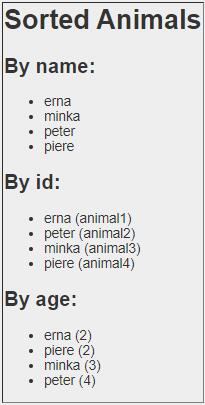
\includegraphics[scale=0.8]{2.jpg}
\end{center}

那么,.xsl文件可以这样写:

\begin{minted}{xml}
<?xml version="1.0" encoding="UTF-8"?>

<xsl:stylesheet version="1.0"
    xmlns:xsl="http://www.w3.org/1999/XSL/Transform"
>

	<xsl:template match="/">

		<html>
			<!--这一行可以省略,这是用来防止浏览器预留缓存的-->
			<meta http-equiv="cache-control" content="no-cache, no-store"/>
			<body>
				<h1>Sorted Animals</h1>
				<h2>By name:</h2>
				<ul>
					<xsl:apply-templates select="zoo/zoo_animal/name">
						<xsl:with-param name="q" select="'name'"/>
						<!--排序根据name字母升序-->
						<xsl:sort data-type="text/qname" order="incending"/>
					</xsl:apply-templates>
				</ul>
				<h2>By id:</h2>
				<ul>
					<xsl:apply-templates select="zoo/zoo_animal[@id]/name">
						<xsl:with-param name="q" select="'id'"/>
						<!--排序根据@id数字升序-->
						<xsl:sort data-type="number" order="incending"/>
					</xsl:apply-templates>
				</ul>
				<h2>By age:</h2>
				<ul>
					<xsl:apply-templates select="zoo/zoo_animal/age">
						<xsl:with-param name="q" select="'age'"/>
						<!--排序根据age数字升序-->
						<xsl:sort data-type="number" order="incending"/>
					</xsl:apply-templates>
				</ul>
			</body>
		</html>
	</xsl:template>

	<xsl:template match="*" >
		<!--根据传进来的字符串选择对应的处理方式-->
		<xsl:param name="q"/>
		<xsl:if test=".!=''">
			<li>
				<xsl:choose>
					<xsl:when test="$q='name'">
						<xsl:value-of select="."/>
					</xsl:when>
					<xsl:when test="$q='id'">
						<xsl:value-of select="."/>
						(<xsl:value-of select="./../@id"/>)
					</xsl:when>
					<xsl:when test="$q='age'">
						<xsl:value-of select="./../name"/>
						(<xsl:value-of select="."/>)
					</xsl:when>
				</xsl:choose>
			</li>
		</xsl:if>
	</xsl:template>

</xsl:stylesheet>
\end{minted}

\subsection{XSLT 实例2}

在.xsl中可以利用模板实现递归操作。

已知numbers.xml:

\begin{minted}{xml}
<?xml version="1.0" encoding="utf-8"?>
<?xml-stylesheet type="text/xsl" href="task12.xsl"?>
<numbers>
	<number value="8"/>
	<number value="3"/>
	...
</numbers>
\end{minted}

期望根据其value值有以下输出:
例如8输出8次,3输出3次。

\begin{center}
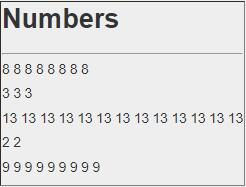
\includegraphics[scale=0.8]{3.jpg}
\end{center}

那么可能的.xsl文件如下:
\begin{minted}{xml}
<?xml version="1.0" encoding="UTF-8"?>
<xsl:stylesheet version="1.0"
    xmlns:xsl="http://www.w3.org/1999/XSL/Transform"
>
	<xsl:template match="/">
		<html>
			<meta http-equiv="cache-control" content="no-cache, no-store"></meta>
			<body>
				<h1>Numbers</h1>
				<hr/>
				<xsl:for-each select="numbers/number">
					<p>
						<!--在此处使用递归,
						v为固定的@value值,
						i初始为1,i记录递归次数-->
						<xsl:call-template name="recv">
							<xsl:with-param name="v" select="@value"/>
							<xsl:with-param name="i" select="1"/>
						</xsl:call-template>
					</p>
				</xsl:for-each>
			</body>
		</html>
	</xsl:template>

	<xsl:template name="recv">
		<xsl:param name="v"/>
		<xsl:param name="i"/>
		<!--判断当前递归次数,若i<=value,说明递归次数未达到value值
			若i>value,说明递归结束。
			每次递归时,将i值+1  -->
		<xsl:if test="$i &lt;= $v">
			<xsl:value-of select="$v"/>
			<xsl:text> </xsl:text>
			<xsl:call-template name="recv">
				<xsl:with-param name="v" select="$v"/>
				<xsl:with-param name="i" select="$i + 1"/>
			</xsl:call-template>
		</xsl:if>
	</xsl:template>
</xsl:stylesheet>
\end{minted}

\subsection{XSLT 实例3}

用xsl:attribute来为标签添加属性。本题为标签添加了css样式

已知candidates.xml形如:

\begin{minted}{xml}
<?xml version="1.0" encoding="iso-8859-1"?>
<?xml-stylesheet type="text/xsl" href="task13.xsl"?>
<evaluation>
	<candidate>
		<name>Peter</name>
		<points>67</points>
	</candidate>
	...
</evaluation>
\end{minted}

期望的输出如下图:

\begin{center}
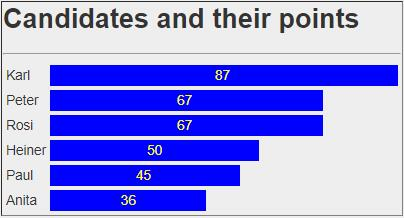
\includegraphics[scale=0.8]{4.jpg}
\end{center}

那么,可能的.xsl文件如下:

\begin{minted}{xml}
<?xml version="1.0" encoding="UTF-8"?>
<xsl:stylesheet version="1.0"
    xmlns:xsl="http://www.w3.org/1999/XSL/Transform"
>
	<xsl:template match="/">
		<html>
			<meta http-equiv="cache-control" content="no-cache, no-store"></meta>
			<body>
				<h1>Candidates and their points</h1>
				<hr/>
				<xsl:for-each select="//candidate">
					<p >
						<div class="lab"><xsl:value-of select="name"/></div>
						<div class="lab1" align="left">
							<!--在此处,为div标签附加一个内联的css样式
								关键字为style-->
							<xsl:attribute name="style">
								<xsl:text>width:</xsl:text>
								<xsl:value-of select="points"/>
								<xsl:text>px;background-color:blue;
									color:white;text-align:center;
								</xsl:text>
							</xsl:attribute>
							<xsl:value-of select="points"/>
						</div>
					</p>
				</xsl:for-each>
			</body>
			<style>
				.lab{
					display: inline-block;
					width:60px;
				}
				.lab1{
					display: inline-block;
				}
			</style>
		</html>
	</xsl:template>
</xsl:stylesheet>
\end{minted}

\subsection{XSLT 实例4}

通过XSLT不光能输出XML文件,也可以输出LaTex文件:

已知table.xml文件形如:

\begin{minted}{xml}
<?xml version="1.0" encoding="utf-8"?>
<?xml-stylesheet type="text/xsl" href="task14.xsl"?>
<table>
	<row>
		<column>Reiner</column>
		<column>Liebig</column>
		<column>52612</column>
		<column>Leipzig</column>
	</row>
	...
</table>
\end{minted}

期望输出的LaTex生成样子如下:

\begin{center}

\includegraphics[scale=0.8]{5.jpg}
\end{center}

那么,可能的.xsl文件如下:

\begin{minted}{xml}
<?xml version="1.0" encoding="UTF-8"?>
<xsl:stylesheet version="1.0"
    xmlns:xsl="http://www.w3.org/1999/XSL/Transform"
>
<xsl:template match="/">
\documentclass{article}
\usepackage[utf-8]{inputenc}
\usepackage{ngerman}
\pagestyle{empty}
\begin{document}
\begin{tabular}{|c|c|c|c|}
\hline
<xsl:for-each select="table/row">
    <xsl:for-each select="column">
		<!--通过position()判断当前元素位置,其从0开始
			前三个元素在后面添加符号&,最后一个元素后面添加\\ \hline-->
        <xsl:if test="position() &lt; 4">
            <xsl:value-of select="."/>
			<!--此处用了CDATA方法,因为&会出现转义,这不是我们期望的-->
            <xsl:text disable-output-escaping="yes"><![CDATA[&]]></xsl:text>
        </xsl:if>
        <xsl:if test="position() = 4">
            <xsl:value-of select="."/><xsl:text>\\ \hline </xsl:text>
        </xsl:if>
    </xsl:for-each>
</xsl:for-each>
\end{tabular}
\end{document}
</xsl:template>
</xsl:stylesheet>
\end{minted}

\subsection{XSLT 实例5}

不通过when-otherwise来访问每一个标签,而是通过xsl:element来创建新的元素,以此显示期望的结果。

已知article.xml文件如下:

\begin{minted}{xml}
<?xml version="1.0" encoding="utf-8" ?>
<?xml-stylesheet type="text/xsl" href="task15.xsl"?>
<article title="Rockville opens new Library">
  <text style="h1">Rockville opens new Library</text>
  <text style="p">On saturday the major of Rockville 
	  officially opened the city's new library.</text>
  <text style="hr"></text>
  <text style="h2">3 year construction finally finished</text>
  <text style="p">The building, which had been under 
	  construction for 3 years had been recently finished 
	  and now houses the city's new library.</text>
  <text style="blockquote">This is a huge success for Rockville.</text>
  <text style="p">The major called the opening of the 
	  library a huge success during the opening ceremony.</text>
  <text style="i">Written by Joice A. Price, leading journalist 
	  of the Rockville Daily since 1967.</text>
</article>
\end{minted}

期望的输出形如下图:

\begin{center}
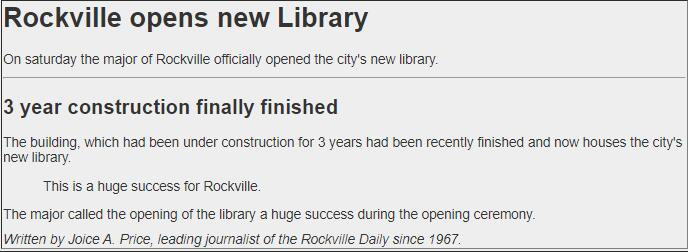
\includegraphics[scale=0.8]{6.jpg}
\end{center}

可能的.xsl文件如下:

\begin{minted}{xml}
<?xml version="1.0" encoding="UTF-8"?>
<xsl:stylesheet version="1.0"
    xmlns:xsl="http://www.w3.org/1999/XSL/Transform"
>
	<xsl:template match="/">
		<html>
			<meta http-equiv="cache-control" content="no-cache, no-store"></meta>
			<xsl:for-each select="article/text">
				<xsl:apply-templates select=".">
					<!--提取style中的字符串,传给模板-->
					<xsl:with-param name="sty" select="@style"/>
				</xsl:apply-templates>
				<br/>
			</xsl:for-each>
		</html>
	</xsl:template>

	<xsl:template match="//text">
		<xsl:param name="sty"/>
		<!--在模板中,将获取到的@style的值设定为name的值,并输出下面这个element-->
		<xsl:element name="{$sty}">
			<xsl:value-of select="."/>
		</xsl:element>
	</xsl:template>
</xsl:stylesheet>
\end{minted}

\section{lb4: RDF (.rdf), SPARQL, OWL}

\subsection{概念}

判断:

F1: What of these are not goals of linked data? 哪些不是关联数据的目标?

\indent\indent Increasing reusability 增加可重用性

\indent\indent Combining multiple data sets 组合多个数据集

\indent\indent Reducing file size 减小文件大小($\checkmark$)

\indent\indent Allowing inference 允许推理

F2: Linked data uses URIs as unique identifiers for entities 链接数据使用 URI 作为实体的唯一标识符($\checkmark$)

F3: RDF...

\indent\indent provides a clear hierarchy 提供了清晰的层次结构

\indent\indent allows blank nodes without a URI 允许没有 URI 的空白节点($\checkmark$)

\indent\indent requires the use of a schema 需要使用模式

\indent\indent expresses information as subject-adjective-predicate triples 将信息表达为主-形容词-谓词三元组

F4: SPARQL...

\indent\indent is a read-only query language 是一种只读查询语言

\indent\indent uses placeholders to represent unkown entities or predicates 使用占位符来表示未知的实体或谓词($\checkmark$)

\indent\indent uses the same syntax as SQL 使用与 SQL 相同的语法

\indent\indent queries information from a single graph 从单个图中查询信息

F5: Inference 推理

\indent\indent uses RDF Schema classes 使用 RDF Schema 类

\indent\indent is implemented through reasoners 是通过推理器实现的($\checkmark$)

\indent\indent adds triples not explicitly stated to the graph 将未明确说明的三元组添加到图中($\checkmark$)

\indent\indent requires OWL 需要 OWL

\subsection{RDF}

XML defines a flexible way of storing structured data and as such allows data to be structured very differently. Consequently, data from various sources usually can't be combined easily, as the information is structured differently.  RDF tries to solve this by providing a simple yet flexible way to store arbitrary information. It achieves this by breaking down information into fundamental statements, consisting of a subject, predicate and an object. These statements are therefore called triples. RDF uses URIs to refer to entities and predicates. Different files containing RDF can then be easily combined, and references to same things can be identified, as they use the same URIs.

XML 定义了一种存储结构化数据的灵活方式,因此允许数据的结构非常不同。 
因此,\textbf{来自不同来源}的数据通常无法轻松组合,因为信息的结构不同。 
\textbf{RDF 试图通过提供一种简单而灵活的方式来存储任意信息来解决这个问题。}
它通过将信息分解为由\textbf{主语、谓语和宾语}组成的基本陈述来实现这一点。 
因此,这些语句被称为三元组。 
RDF 使用 URI 来引用实体和谓词。 然后可以轻松组合包含 RDF 的不同文件,并且\textbf{可以识别对相同事物的引用},
因为它们使用相同的 URI。

\subsection{RDF 实例}

已知3个.rdf文件author.rdf/books.rdf/translators.rdf。
期望通过RDF来找到如下图的关系,并显示出来。

\begin{center}
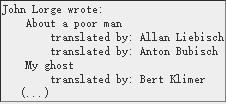
\includegraphics[scale=1]{7.jpg}
\end{center}

.rdf文件属下:

\begin{minted}{xml}
<!--authors.rdf-->
<rdf:RDF
    xmlns:lit="http://example.org/lit#"
    xmlns:rdf="http://www.w3.org/1999/02/22-rdf-syntax-ns#" > 
  <rdf:Description rdf:about="http://example.org/lit#author0">
    <lit:hasWritten rdf:resource="http://example.org/lit#book12"/>
    <lit:hasWritten rdf:resource="http://example.org/lit#book3"/>
    <lit:hasWritten rdf:resource="http://example.org/lit#book0"/>
    <lit:authorName>John Lorge</lit:authorName>
  </rdf:Description>
  <rdf:Description rdf:about="http://example.org/lit#author2">
    <lit:hasWritten rdf:resource="http://example.org/lit#book4"/>
    <lit:hasWritten rdf:resource="http://example.org/lit#book1"/>
    <lit:authorName>Tony Cash</lit:authorName>
  </rdf:Description>
  ...
</rdf:RDF>

<!--books.rdf-->
<rdf:RDF
    xmlns:lit="http://example.org/lit#"
    xmlns:rdf="http://www.w3.org/1999/02/22-rdf-syntax-ns#" > 
  <rdf:Description rdf:about="http://example.org/lit#book4">
    <lit:bookName>The writer</lit:bookName>
  </rdf:Description>
  ...
</rdf:RDF>

<!--translators.rdf-->
<rdf:RDF
    xmlns:lit="http://example.org/lit#"
    xmlns:rdf="http://www.w3.org/1999/02/22-rdf-syntax-ns#" > 
  <rdf:Description rdf:about="http://example.org/lit#author48">
    <lit:hasTranslated rdf:resource="http://example.org/lit#book14"/>
    <lit:hasTranslated rdf:resource="http://example.org/lit#book17"/>
    <lit:authorName>Reiner Klumpatsch</lit:authorName>
  </rdf:Description>
  ...
</rdf:RDF>
\end{minted}

那么,可能的.py文件如下:

\begin{minted}{python}
import rdflib
g = rdflib.Graph()
g1 = rdflib.Graph()
g2 = rdflib.Graph()

g.parse("translators.rdf")
g1.parse("authors.rdf")
g2.parse("books.rdf")

g = g + g1 + g2

authorPaar = {}     # 作者名字URI : 作者实际名字
authorAndBook = {}  # 作者名字 : [书]
bookPaar = {}       # 书名字URI : 书实际名字
transPaar = {}      # 翻译名字URI : 翻译实际名字
transAndBook = {}   # 翻译名字 : [书]

# s,p,o为由RDF得到的三元组,
# 例如当p为<http://example.org/lit#authorName>时,三元组如下:
# <http://example.org/lit#author48> 	<--主语 subject
# <http://example.org/lit#authorName>   <--谓语 predicate
# Reiner Klumpatsch						<--宾语 object
for s,p,o in g:
    if "authorName" in str(p) and str(p) not in authorPaar:
        authorPaar[str(s)] = str(o)
    if "hasWritten" in str(p):
        if str(s) not in authorAndBook:
            authorAndBook[str(s)] = []
        authorAndBook[str(s)].append(str(o))
    if "bookName" in str(p):
        bookPaar[str(s)] = str(o)
    if "authorName" in str(p) and str(p) not in transPaar:
        transPaar[str(s)] = str(o)
    if "hasTranslated" in str(p):
        if str(s) not in transAndBook:
            transAndBook[str(s)] = []
        transAndBook[str(s)].append(str(o))
tempAB = {}     # 将authorAndBook的key从URI格式替换为作者实际名字
for i in authorAndBook.keys():
    tempAB[authorPaar[i]] = authorAndBook[i]
authorAndBook = tempAB
# 将authorAndBook中的value内书名字URI替换为书实际名字
for i in authorAndBook.keys():
    tempBook = []
    for j in authorAndBook[i]:
        tempBook.append(bookPaar[j])
        authorAndBook[i] = tempBook  
# 将transAndBook的key从URI格式名字替换为翻译实际名字
tempTB = {}
for i in transAndBook.keys():
    tempTB[transPaar[i]] = transAndBook[i]
transAndBook = tempTB
# 将transAndBook的value内书名字URI替换为实际书名字
for i in transAndBook.keys():
    tempBook = []
    for j in transAndBook[i]:
        tempBook.append(bookPaar[j])
        transAndBook[i] = tempBook
# 函数,根据书名找到其翻译者,返回翻译者列表
def findTranslator(transAndBook, bookName):
    nameList = []
    for i in transAndBook.keys():
        if bookName in transAndBook[i]:
            nameList.append(i)
    return nameList
# 输出
for i in authorAndBook.keys():
    print(i + "wrote:")
    for j in authorAndBook[i]:
        print("\t" + j)
        nameList = findTranslator(transAndBook, j)
        for k in range(len(nameList)):
            print("\t\t translated by: " + nameList[k])
\end{minted}

\subsection{SPARQL}

Altough working with RDF data via an application is possible, it can become rather tedious, especially since executing a number of different queries require rewriting the application several times. An easier option to get information from a RDF graph is SPARQL. As it is a query language it is somewhat similar to SQL, which is used to query relational databases, but instead for RDF graphs.

尽管通过应用程序处理 RDF 数据是可能的,但它会变得相当乏味,
尤其是因为执行许多不同的查询需要多次重写应用程序。 
从 RDF 图获取信息的一个更简单的选择是 SPARQL。 
由于它是一种查询语言,它有点类似于 SQL,后者用于查询关系数据库,但用于查询 RDF 图。

SPARQL queries describe a kind of pattern containing placeholders, that the RDF graph is then searched for. For matching sub-graphs the placeholders match specific URIs, which are returned as the results of the query, depending on the SELECT statement

SPARQL 查询描述了一种包含占位符的模式,然后搜索 RDF 图。 
对于匹配子图,占位符匹配特定的 URI,这些 URI 作为查询结果返回,具体取决于 SELECT 语句

\subsection{SPARQL 实例1}

\begin{minted}{python}
# 列出作者名字、书、翻译者,形如:
# | name            | the_book_name        | translator     |
# ===========================================================
# | "John Lorge"    | "About a poor man"   | Renate Koller  |
# | "Tony Cash"     | "The writer"         | Anton Bubisch  |
#  (.......................................................)
# | "Allen Weak"    | "The Castle"         | Allan Liebisch 
import rdflib

g1 = rdflib.Graph()
g2 = rdflib.Graph()
g3 = rdflib.Graph()
g1.parse("authors.rdf")
g2.parse("books.rdf")
g3.parse("translators.rdf")
g1 = g1 + g2 + g3

qres = g1.query(
    """
        PREFIX rdf:<http://example.org/lit#>
        SELECT DISTINCT ?name ?the_book_name ?translator WHERE{
            ?author rdf:hasWritten ?book.
            ?author rdf:authorName ?name.
            
            ?Translator rdf:hasTranslated ?book.
            ?Translator rdf:authorName ?translator.
            ?book rdf:bookName ?the_book_name.
        }
    """
)
data = []
print("{:<30} {:<30} {:<30}".format("name","the_book_name","translator"))
for row in qres:
    data.append(row)
for v in data:
    name, the_book_name, translator = v
    print("{:<30} {:<30} {:<30}".format(name, the_book_name, translator))
\end{minted}

\subsection{SPARQL 实例2}

\begin{minted}{python}
# 列出所有书名含有"about"的,或者作者住在Magdeburg的,形如
# ---------------------------------------
# | name           | the_book_name      |
# =======================================
# | "John Lorge"   | "About a poor man" |
# | "Lionel Hurby" | "About us"         |
# | "Clara Heller" | "The dirty meal"   |
# | "Clara Heller" | "The hammer"       |
# | "Clara Heller" | "Let's Dance"      |
# ---------------------------------------
import rdflib
g1 = rdflib.Graph()
g2 = rdflib.Graph()
g3 = rdflib.Graph()
g1.parse("authors.rdf")
g2.parse("books.rdf")
g3.parse("locations.rdf")
g1 = g1 + g2 + g3
qres1 = g1.query(
    """
		PREFIX rdf: <http://example.org/lit#>
		SELECT DISTINCT ?name ?the_book_name WHERE {
		?author rdf:authorName ?name.
		?author rdf:hasWritten ?book.
		?book rdf:bookName ?the_book_name.
		?author rdf:livesIn ?location
			FILTER (regex(?the_book_name, "about", "i") || 
				regex(?location, "Magdeburg", "i"))
		}
    """
)
for row in qres1:
    print(row[0] + " |" + row[1])
\end{minted}

\subsection{SPARQL 实例3}

\begin{minted}{python}
# 列出所有作者,并显示他们写的书或翻译的书,形如:
# ---------------------------------------------------------------------
# | Autoren             | written_book_name    | translated_book_name |
# =====================================================================
# | "Donald Meier"      |                      | "The better way"     |
# | "Donald Meier"      |                      | "The wild west"      |
# | "Laure Castel"      | "Sounds good"        |                      |
# | "Laure Castel"      | "Harry, the tramp"   |                      |
# | "Laure Castel"      | "What did you do?"   |                      |
# | "Ilona Leonhadt"    |                      | "About us"           |
# | "Ilona Leonhadt"    |                      | "Oh, oh oh..."       |
#   (................................................................)
# | "Reiner Klumpatsch" |                      | "The daisy killer"   |
# | "Reiner Klumpatsch" |                      | "Hold on"            |
# ---------------------------------------------------------------------
import rdflib
g1 = rdflib.Graph()
g2 = rdflib.Graph()
g3 = rdflib.Graph()
g1.parse("authors.rdf")
g2.parse("books.rdf")
g3.parse("translators.rdf")
g1 = g1 + g2 + g3
qres1 = g1.query(
    """
		PREFIX rdf: <http://example.org/lit#>
		SELECT DISTINCT ?Author ?written_book_name ?translated_book_name WHERE {
			?author rdf:authorName ?Author.
			{
				?author rdf:hasWritten ?book.
				?book rdf:bookName ?written_book_name.
			}
			UNION
			{
				?author rdf:hasTranslated ?book.
				?book rdf:bookName ?translated_book_name
			}
		}
    """
)
for row in qres1:
    print(row[0] + " | " + row[1]+" | "+ row[2])
\end{minted}

\subsection{OWL}

Humans have the ability to understand the information within an RDF graph and also come to conclusions about information that is not stated explicitly, due to previous experience and knowledge. Computers however are unable to work with such implicit knowledge since they lack this pre-knowledge. OWL and similar tools allow an application to gain such implicit pre-knowledge, and turn it in to explicit statements (triples). This works by describing properties of certain relationships between entities.

由于先前的经验和知识,人类有能力理解 RDF 图中的信息,并且还可以对未明确说明的信息得出结论。 
然而,计算机无法使用这种隐含的知识,因为它们缺乏这种先验知识。 
OWL 和类似工具允许应用程序获得这种隐含的预知识,并将其转化为显式语句(三元组)。 
这通过描述实体之间某些关系的属性来工作。

Before an application can work with the implicit information, it needs to be made explicit in a process called Reasoning or Inference. In Python this can be achieved with the module owlrl:

在应用程序可以使用隐式信息之前,需要在称为推理或推理的过程中使其显式。 
在 Python 中,这可以通过 owlrl 模块来实现:

\subsection{OWL 实例1}

已知Schulpers.owl和Schulpersonal.rdf文件。

\begin{minted}{xml}
<!--Schulpers.owl-->
<?xml version="1.0"?>
<!DOCTYPE rdf:RDF [
    <!ENTITY owl "http://www.w3.org/2002/07/owl#" >
]>
<rdf:RDF
    xmlns:rdf="http://www.w3.org/1999/02/22-rdf-syntax-ns#"
    xmlns:xsd="http://www.w3.org/2001/XMLSchema#"
    xmlns:rdfs="http://www.w3.org/2000/01/rdf-schema#"
    xmlns:owl="http://www.w3.org/2002/07/owl#"
  	xml:base="http://example.org/personal/per">
	<owl:Class rdf:ID="person"/>
	<owl:Class rdf:ID="employee">
		<rdfs:subClassOf rdf:resource="#person"/>
	</owl:Class>
	<owl:Class rdf:ID="student">
		<rdfs:subClassOf rdf:resource="#person"/>
	</owl:Class>
	<owl:Class rdf:ID="caretaker">
		<rdfs:subClassOf rdf:resource="#employee"/>
	</owl:Class>
	<owl:Class rdf:ID="teacher">
		<rdfs:subClassOf rdf:resource="#employee"/>
	</owl:Class>
	<owl:ObjectProperty rdf:ID="teaches">
		<rdfs:domain rdf:resource="#teacher"/>
		<rdfs:range rdf:resource="#student"/>
	</owl:ObjectProperty>
	<owl:ObjectProperty rdf:ID="isRelative"/>
	<owl:ObjectProperty rdf:ID="isFather">
		<rdfs:subPropertyOf rdf:resource="#isRelative"/>
		<rdfs:range rdf:resource="#person"/>
		<owl:inverseOf rdf:resource="#isChild"/>
		<rdfs:domain rdf:resource="#person"/>
	</owl:ObjectProperty>
	<owl:ObjectProperty rdf:ID="isChild">
		<rdfs:domain rdf:resource="#person"/>
		<rdfs:range rdf:resource="#person"/>
		<owl:inverseOf rdf:resource="#isFather"/>
		<rdfs:subPropertyOf rdf:resource="#isRelative"/>
	</owl:ObjectProperty>
	<owl:ObjectProperty rdf:ID="isBrother">
		<rdf:type rdf:resource="&owl;TransitiveProperty"/>
		<rdf:type rdf:resource="&owl;SymmetricProperty"/>
		<rdfs:subPropertyOf rdf:resource="#isRelative"/>
	</owl:ObjectProperty>
</rdf:RDF>
\end{minted}

\begin{minted}{xml}
<!--Schulpersonal.rdf-->
<?xml version="1.0"?>
<!DOCTYPE rdf:RDF [
    <!ENTITY per "http://example.org/personal/per#" >
]>
<rdf:RDF
    xmlns:per="http://example.org/personal/per#"
    xmlns:rdf="http://www.w3.org/1999/02/22-rdf-syntax-ns#"
    xmlns:rdfs="http://www.w3.org/2000/01/rdf-schema"
    xmlns:owl="http://www.w3.org/2002/07/owl#"
    xmlns:daml="http://www.daml.org/2001/03/daml+oil#" > 
	<rdf:Description rdf:about="&per;bernd_liebisch">
		<rdf:type rdf:resource="&per;student"/>
	</rdf:Description>
	<rdf:Description rdf:about="&per;paul_linke">
		<per:isFather rdf:resource="&per;heiner_lederer"/>
		<per:isBrother rdf:resource="&per;andreas_hilbert"/>
		<per:teaches rdf:resource="&per;heiner_lederer"/>
		<per:teaches rdf:resource="&per;bernd_liebisch"/>
		<rdf:type rdf:resource="&per;teacher"/>
	</rdf:Description>
	<rdf:Description rdf:about="&per;peter_meier">
		<rdf:type rdf:resource="&per;teacher"/>
	</rdf:Description>
	<rdf:Description rdf:about="&per;alfred_lober">
		<rdf:type rdf:resource="&per;student"/>
	</rdf:Description>
	<rdf:Description rdf:about="&per;caretaker1">
		<per:isFather rdf:resource="&per;alfred_lober"/>
		<owl:sameAs rdf:resource="&per;hans_breuer"/>
		<rdf:type rdf:resource="&per;caretaker"/>
	</rdf:Description>
	<rdf:Description rdf:about="&per;heiner_lederer">
		<rdf:type rdf:resource="&per;student"/>
	</rdf:Description>
	<per:teacher rdf:about="&per;andreas_hilbert">
		<per:isBrother rdf:resource="&per;peter_meier"/>
		<per:teaches rdf:resource="&per;alfred_lober"/>
		<per:teaches rdf:resource="&per;bernd_liebisch"/>
	</per:teacher>
</rdf:RDF>
\end{minted}

通过teacher找到所有的brother,而且brother不能是student。Find all the brothers among the teachers (but not the students)!

可能的.py如下:

\begin{minted}{python}
import rdflib
import owlrl

graph = rdflib.Graph()
graph.parse("Schulpersonal.rdf")
graph.parse("Schulpers.owl")
owlrl.DeductiveClosure(owlrl.OWLRL_Semantics).expand(graph)

per = rdflib.Namespace("http://example.org/personal/per#")
print("Brother among Teachers, and not a strudent")
for s in graph.subjects(rdflib.RDF.type,per.teacher):
    for b in graph.objects(s,per.isBrother):
        if (s != b) and b not in [ b1 for b1 in graph.subjects(b, per.student)]:
            print(s, "is brother of", b)
\end{minted}

\subsection{OWL 实例2}

判断一个caretaker的身份是否是teacher/student/empoloyee/person

输出如下:
\begin{center}
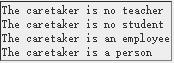
\includegraphics[scale=1]{8.jpg}
\end{center}

可能的.py如下:

\begin{minted}{python}
import rdflib
import owlrl

graph = rdflib.Graph()
graph.parse("Schulpersonal.rdf")
graph.parse("Schulpers.owl")
owlrl.DeductiveClosure(owlrl.OWLRL_Semantics).expand(graph)

per = rdflib.Namespace("http://example.org/personal/per#")

print("caretaker is a Teacher and/or a student and/or an Empoloyee and/or a Person")
# 找到所有的caretaker
for s in graph.subjects(rdflib.RDF.type,per.caretaker):
    mark = [0,0,0,0]
    workList = ["student","teacher","employee","person"]   
    # 打印当前caretaker的名字
    print(str.replace(str(s),str(per),""))
    # 对于当前的caretaker,根据名字找到其工作/身份
    for w in graph.objects(s, rdflib.RDF.type):
        work = str.replace(str(w),str(per),"")
        if work == "student":
            mark[0] = 1
        if work == "teacher":
            mark[1] = 1
        if work == "employee":
            mark[2] = 1
        if work == "person":
            mark[3] = 1
    # 根据找到的身份,打印相关信息
    for i in range(4):
        if mark[i] == 0:
            print("\t caretaker is no " + workList[i])
        if mark[i] == 1 and i == 2:
            print("\t caretaker is an " + workList[i])  
        if mark[i] == 1 and i != 2:
            print("\t caretaker is a " + workList[i]) 
\end{minted}

\section{lb5: RDF in the Web}

\subsection{概念}

判断:

F1: How can RDF be integrated with HTML? RDF如何与HTML结合?

\indent\indent RDFa ($\checkmark$)

\indent\indent GRDDL ($\checkmark$)

\indent\indent text/turtle

\indent\indent Microformats ($\checkmark$)

F2: Direct inclusion of RDF breaks HTML validity. 直接包含 RDF 会破坏 HTML 的有效性。($\checkmark$)

F3: RDF Serialization is the process of... RDF序列化是...的过程

\indent\indent translating XML data to RDF 将 XML 数据转换为 RDF

\indent\indent validating RDF data to a specific Schema 验证 RDF 数据到一个特定的 Schema

\indent\indent ordering the triples in an RDF graph 对 RDF 图中的三元组进行排序

\indent\indent writing RDF data in a specific file format 以特定文件格式写入 RDF 数据($\checkmark$)

F4: Which type of RDF-HTML integration is shown here?
这里显示了哪种类型的 RDF-HTML 集成?
\begin{minted}{html}
<html>
	<head>
		<title>Staff</title>
	</head>
	<body vocab="http://www.w3.org/2006/vcard/ns#">
		<h1>Staff</h1>
		<p>These are the people that made Enviro Architectural Designs 
			what it is today:</p>
		<div about="http://example.org/staff#phoover" typeof="Individual">
			<h2 rel="hasName">
				<span property="given-name">Patrick</span>
				<span property="family-name">Hoover</span>
			</h2>
			<p>Patrick (57<span style="display:none" property="bday">1965</span>) 
				is Enviro's 
				<span property="title">International Marketing Supervisor</span>.
			</p>
			<table>
				<tr>
					<td>Mail:</td>
					<td><a href="mailto:PatrickHoover@example.org" 
						property="hasEmail">PatrickHoover@example.org</a></td>
				</tr>
				<tr>
					<td>Address:</td>
					<td rel="adr"><span property="street-address">
						Budapester Strasse 5</span>,
						<span property="postal-code">24606</span> 
						<span property="locality">Trappenkamp</span>
					</td>
				</tr>
			</table>
		</div>
	</body>
</html>
\end{minted}

\indent\indent Microformats

\indent\indent JSON-LD

\indent\indent GRDDL

\indent\indent RDFa ($\checkmark$)

F5: For which use cases would you integrate RDF into HTML? 对于哪些用例,您会将 RDF 集成到 HTML 中?

\indent\indent As JSON alternative in Web Frontends 作为 Web 前端中的 JSON 替代方案

\indent\indent To render vector graphics in the browser 在浏览器中渲染矢量图形

\indent\indent SEO (Search Engine Optimization) SEO(搜索引擎优化)($\checkmark$)

\indent\indent To support human and machine access 支持人机访问($\checkmark$)

\subsection{how can RDF be combined with HTML RDF如何与HTML结合?}

\subsubsection{Idea 1}

\noindent\textbf{1. HTML 1.x}: 使用元数据Metadata。

这种情况下,需要对不同的标签分别进行讨论。

In this case, the different tags need to be discussed separately.

问题在于:seen and unseen metadata of a document (extremely hard to maintain 极难维护, see ex. "WSDL Description vs. Definition")

\noindent\textbf{2. HTML <link>}: 

元数据放在外部文件中。(与 HTML 资源的弱连接)Metadata/RDF in an external resource.(weak connection to an HTML resource)

\begin{minted}{xml}
<head> 
	<link rel="meta" type="application/rdf+xml" href="meta.rdf"/> 
</head>
\end{minted}

\noindent\textbf{3. HTML <a>}:

元数据放在外部文件中。(与 HTML 资源的弱连接)Metadata/RDF in an external resource.(weak connection to an HTML resource)

\begin{minted}{xml}
	<body> 
		<a rel="meta" type="application/rdf+xml" href="meta.rdf">Text</a>
		...
\end{minted}

\subsubsection{Idea 2: XML/RDF in XHTML}

用XML/RDF in XHTML的方法。

obvious approach - validation is impossible (XHTML-DTDs)

显而易见的方法 - 验证是不可能的

\begin{minted}{xml}
<head>
	<title>Beispiel</title> 
	<rdf:RDF
		xmlns:rdf="http://www.w3.org/1999/0…" 
		xmlns:dc="http://purl.org/dc/elements/1.1/"
	>
		<rdf:Description rdf:about="http://example.org/" dc:title="Beispiel"/>
	</rdf:RDF> 
</head>
\end{minted}

\subsubsection{Idea 3: XML/RDF in XHTML comments. XML/RDF in URI scheme}

\noindent\textbf{XML/RDF in XHTML comments}:

HTML comments enable people to provide other people with information about the code - not made for machines

HTML 注释使人们能够向其他人提供有关代码的信息——不是为机器设计的。

\begin{minted}{xml}
<!--<rdf:RDF xmlns="http://web.resource.org/cc/" 
		xmlns:rdf="http://www.w3.org/1999/02/22-rdf-syntax-ns#"
	> 
		<License rdf:about="http://creativecommons.org/licenses/by-ncsa/1.0"> 
			<requires rdf:resource="http://web.resource.org/cc/Attribution" /> 
			<requires rdf:resource="http://web.resource.org/cc/ShareAlike" /> 
			<requires rdf:resource="http://web.resource.org/cc/Notice" /> 
			<prohibits rdf:resource="http://web.resource.org/cc/CommercialUse" /> 
			<permits rdf:resource="http://web.resource.org/cc/Reproduction" /> 
			<permits rdf:resource="http://web.resource.org/cc/Distribution" /> 
			<permits rdf:resource="http://web.resource.org/cc/DerivativeWorks" /> 
		</License> 
	</rdf:RDF> -->
\end{minted}

\noindent\textbf{XML/RDF in URI scheme}:

RFC 2397 defines data as a URI scheme. RFC 2397 将数据定义为 URI 方案。

格式:data:[<MIME-type>][;base64],<data>

例如:
\begin{minted}{xml}
<A SRC="data:application/rdf+xml ;base64; PHJkZjpSREYg....."> Text with metadata</a>
\end{minted}

\subsubsection{Idea 4: Microformats 微格式}

Use existing standards, such as vCard (RFC 2426) and defined (or “standardized”) representation in (X)HTML.

使用现有标准,例如 vCard (RFC 2426) 和 (X)HTML 中定义的(或“标准化”)表示。

例如:
\begin{minted}{xml}
<!--vCard notation 电子名片符号
TEL;TYPE=HOME:+49.123.456789
(X)HTML 中的定义表示-->
<span class="tel">
	<span class="type">home</span>: <span class="value">+49(123) 456789</span> 
</span>
\end{minted}

更具体一些:

\begin{minted}{xml}
<!DOCTYPE html PUBLIC "-//W3C//DTD XHTML 1.0 Transitional//EN" ...>
<html xmlns:"http://www.w3.org/1999/xhtml">
	<head>
		<title>Microformats Beispiel</title>
	</head>
	<body>
		<h1>Willkommen</h1>
		<p>
			Mein Name ist
			<div class="vcard">
				<a class="url fn" href="http://gaedke.com/">Martin Gaedke</a>,
				Sie erreichen mich an der
				<div class="org">TU Chemnitz</div>
				telefonisch unter <br />
				<span class="tel">
					<span class="type">Büro</span>:
					<span class="value">+49(999)123456789</span>
				</span>
				<span class="tel">
					<span class="type">Private</span>:
					<span class="value">+49(999)987654321</span>
				</span>
			</div>
		</p>
	</body>
</html>
\end{minted}

\subsubsection{Idea 5: HyperRDF}

Idea: RDF must be easily extractable by XSLT

理念:RDF 必须易于通过 XSLT 提取

\begin{minted}{xml}
<head id="rel" profile="http://www.w3.org/2000/07/hs78#"> 
	<link id="c" rel="rel:classes" href="http://www.w3.org/2000/07/hs78#" />
\end{minted}

\textbf{Trend: Blending RDF with (X)HTML 趋势:将 RDF 与 (X)HTML 混合}

Seen and unseen metadata is easier to maintain (no data duplicates $\rightarrow$ consistency)

可见和不可见的元数据更易于维护(无数据重复$\rightarrow$一致性)

Different metadata formats $\rightarrow$ Extraction from (X)HTML

不同的元数据格式 $\rightarrow$从 (X)HTML 中提取

Approaches for this approach introduce notation rules to be able to use 
 it together with existing technologies like (X)HTML, CSS etc. 
 (for example, Embedded RDF "."-notation in the Head Element and 
 "-"-body for schema declarations)

这种方法的方法引入了符号规则,以便能够将其与 (X)HTML、CSS 等现有技术一起使用
(例如,Head Element 中的嵌入式 RDF "."-notation 和模式声明中的"-"-body )

采用这种方法的有:Microformats, Embedded RDF (is replaced by RDFa), GRDDL, RDFa

\subsection{GRDDL}

GRDDL: Gleaning Resource Descriptions from Dialects of Languages 从语言方言中收集资源描述

GRDDL is a mechanism of obtaining RDF data from XML documents (especially XHTML documents)

GRDDL 是一种从 XML 文档(尤其是 XHTML 文档)中获取 RDF 数据的机制

Thereby, authors can link their documents to a transformation algorithm (especially XSLT) by using a link element

因此,作者可以通过使用链接元素将他们的文档链接到转换算法(尤其是 XSLT)

GRDDL-aware agents can execute the transformation algorithm and process the retrieved RDF data

GRDDL 感知代理可以执行转换算法并处理检索到的 RDF 数据

\begin{minted}{xml}
<!DOCTYPE html PUBLIC "-//W3C//DTD XHTML 1.1//EN"
 "http://www.w3.org/TR/xhtml11/DTD/xhtml11.dtd">
<html xmlns:"http://www.w3.org/1999/xhtml"
	xml:lang="en" lang="en">
	<!--profile关键字用于描述文档使用了某种元数据方案-->
	<!--Profile is used to describe that the document 
		uses a certain metadata scheme-->
	<head profile="http://www.w3.org/2003/g/data-view">
		<title>My GRDDL-Demo Page</title>
		<!--XHTML with GRDDL
			Search for a link element with a transformation, 
			then load the transformation
			搜索带有转换的链接元素,然后加载转换
		-->
		<link rel="transformation" href="http://www.w3.org/2002/12/cal/glean-hcal"/>
	</head>
	<body>...</body>
</html>
<!--通过这个转换,能得到.rdf文件内容形如:
<rdf:Description rdf:about="...">
	<rdf:subject>Some subject</rdf:subject>
	<dc:date>2006-01-02</dc:date>
</rdf:Description>
-->
\end{minted}

\subsection{RDFa (RDF/A)}

\noindent RDFa (previously called RDF/A): Collection of attributes for layering RDF on XML languages. 用于在 XML 语言上分层 RDF 的属性集合

\noindent\textbf{Focus:}

Extension of Link and Meta elements (by changing/complementing XHTML) Link 和 Meta 元素的扩展(通过更改/补充 XHTML)

\indent\indent i.e. Meta elements can have sub-elements 即元元素可以有子元素

Defines generic attributes to enable metadata for all elements 定义通用属性以启用所有元素的元数据

\indent\indent Similar to microformats - but with explicit metadata attributes 类似于微格式——但具有明确的元数据属性

\textbf{Attributes rel, rev, property} - indicate a new statement whose name is the value of the attribute

\textbf{属性 rel、rev、property} - 表示一个新语句,其名称是属性的值

Subject and object are determined via subject or object resolutions accordingly

主体和客体通过相应的主体或客体决议来确定


\begin{minted}{xml}
<div about="photo1.jpg"> 
	A photo with a name 
	<span property="dc:title">Oe</span> 
	of 
	<a rel="dc:creator" rev="foaf:img" href="http://example.org/"> 
		Schmitt
	</a> 
</div>
<!--其生成对应的RDF为
<photo1.jpg> <dc:title> <Literal:"Oe">
<photo1.jpg> <dc:creator> <http://example.org>
<http://example.org> <foaf:img> <photo1.jpg>
-->
\end{minted}




































































\newpage
\end{document}